\documentclass[11pt]{article}
\usepackage[utf8]{inputenc}\usepackage[T1]{fontenc}\usepackage{lmodern}
\usepackage[margin=1in]{geometry}
\usepackage{microtype}\setlength{\emergencystretch}{3em}
\usepackage{amsmath,amssymb,amsthm,booktabs,graphicx,array,xcolor,enumitem,caption}
\graphicspath{{figures/}}
\usepackage[round]{natbib}
\usepackage[hidelinks]{hyperref}
% AUTO-GENERATED by code/make_macros_ds.py. Do not edit by hand.
\makeatletter
\newcommand{\result}[1]{%
  \expandafter\ifx\csname result@#1\endcsname\relax
    \textbf{??}\PackageWarning{results}{undefined key: #1}%
  \else\csname result@#1\endcsname\fi}
\newcommand{\defresult}[2]{\expandafter\def\csname result@#1\endcsname{#2}}
\makeatother

\defresult{absCorrLocalFirst}{0.0388}   % results/attn_*_{structure,natdiv}.json via ds_stats
\defresult{absCorrLocalLast}{0.0404}   % results/attn_*_{structure,natdiv}.json via ds_stats
\defresult{absFromEmptyFirst}{0.0582}   % results/attn_*_{structure,natdiv}.json via ds_stats
\defresult{absFromEmptyLast}{0.0145}   % results/attn_*_{structure,natdiv}.json via ds_stats
\defresult{absFromOppFirst}{0.0093}   % results/attn_*_{structure,natdiv}.json via ds_stats
\defresult{absFromOppLast}{0.0030}   % results/attn_*_{structure,natdiv}.json via ds_stats
\defresult{absGeometryFirst}{0.0721}   % results/attn_*_{structure,natdiv}.json via ds_stats
\defresult{absGeometryLast}{0.0443}   % results/attn_*_{structure,natdiv}.json via ds_stats
\defresult{absIllegalFirst}{0.2528}   % results/attn_*_{structure,natdiv}.json via ds_stats
\defresult{absIllegalLast}{0.1323}   % results/attn_*_{structure,natdiv}.json via ds_stats
\defresult{absLeavesCheckFirst}{0.0776}   % results/attn_*_{structure,natdiv}.json via ds_stats
\defresult{absLeavesCheckLast}{0.0593}   % results/attn_*_{structure,natdiv}.json via ds_stats
\defresult{absToOwnFirst}{0.0357}   % results/attn_*_{structure,natdiv}.json via ds_stats
\defresult{absToOwnLast}{0.0112}   % results/attn_*_{structure,natdiv}.json via ds_stats
\defresult{acAlignProblems}{0}   % results/adapter_checks.json
\defresult{acAlignSites}{4,081}   % results/adapter_checks.json
\defresult{acAllNano}{all three}   % results/adapter_checks.json
\defresult{acCacheMismatch}{0}   % results/adapter_checks.json
\defresult{acCacheSites}{364}   % results/adapter_checks.json
\defresult{acNanoLegal}{20}   % results/adapter_checks.json
\defresult{acNanoTotal}{20}   % results/adapter_checks.json
\defresult{acOpenLegal}{3}   % results/adapter_checks.json
\defresult{acOpenTotal}{3}   % results/adapter_checks.json
\defresult{acOthLegal}{672}   % results/adapter_checks.json
\defresult{acOthTotal}{672}   % results/adapter_checks.json
\defresult{acRandLegal}{0}   % results/adapter_checks.json
\defresult{acRandTotal}{1}   % results/adapter_checks.json
\defresult{acSanCases}{8}   % results/adapter_checks.json
\defresult{acSanCorrect}{8}   % results/adapter_checks.json
\defresult{acVocab}{32}   % results/adapter_checks.json
\defresult{blkManyK0}{9}   % results/blocker_check.json
\defresult{blkManyN}{9}   % results/blocker_check.json
\defresult{blkN}{28}   % results/blocker_check.json
\defresult{blkOneK1}{18}   % results/blocker_check.json
\defresult{blkOneN}{19}   % results/blocker_check.json
\defresult{capCtlDeep}{0.000}   % results/attn_8L256_s0_entangle.json
\defresult{capGapMax}{+0.033}   % results/attn_8L256_s0_entangle.json
\defresult{capGapMin}{+0.011}   % results/attn_8L256_s0_entangle.json
\defresult{capRandDeep}{0.015}   % results/attn_8L256_s0_entangle.json
\defresult{cgAucActH}{0.608}   % results/chessgpt2_{probe,belief_*,edit_*}.json
\defresult{cgAucActR}{0.552}   % results/chessgpt2_{probe,belief_*,edit_*}.json
\defresult{cgAucAggH}{0.530}   % results/chessgpt2_{probe,belief_*,edit_*}.json
\defresult{cgAucAggR}{0.485}   % results/chessgpt2_{probe,belief_*,edit_*}.json
\defresult{cgAucDiffH}{+0.078}   % results/chessgpt2_{probe,belief_*,edit_*}.json
\defresult{cgAucDiffR}{+0.068}   % results/chessgpt2_{probe,belief_*,edit_*}.json
\defresult{cgBelMisH}{0.038}   % results/chessgpt2_{probe,belief_*,edit_*}.json
\defresult{cgBelMisHHi}{0.073}   % results/chessgpt2_{probe,belief_*,edit_*}.json
\defresult{cgBelMisHLo}{0.008}   % results/chessgpt2_{probe,belief_*,edit_*}.json
\defresult{cgBelMisR}{0.061}   % results/chessgpt2_{probe,belief_*,edit_*}.json
\defresult{cgBelMisRHi}{0.078}   % results/chessgpt2_{probe,belief_*,edit_*}.json
\defresult{cgBelMisRLo}{0.046}   % results/chessgpt2_{probe,belief_*,edit_*}.json
\defresult{cgBelOwnH}{0.122}   % results/chessgpt2_{probe,belief_*,edit_*}.json
\defresult{cgBelOwnHHi}{0.192}   % results/chessgpt2_{probe,belief_*,edit_*}.json
\defresult{cgBelOwnHLo}{0.070}   % results/chessgpt2_{probe,belief_*,edit_*}.json
\defresult{cgBelOwnR}{0.188}   % results/chessgpt2_{probe,belief_*,edit_*}.json
\defresult{cgBelOwnRHi}{0.213}   % results/chessgpt2_{probe,belief_*,edit_*}.json
\defresult{cgBelOwnRLo}{0.160}   % results/chessgpt2_{probe,belief_*,edit_*}.json
\defresult{cgBelRandH}{0.000}   % results/chessgpt2_{probe,belief_*,edit_*}.json
\defresult{cgBelRandHHi}{0.000}   % results/chessgpt2_{probe,belief_*,edit_*}.json
\defresult{cgBelRandHLo}{0.000}   % results/chessgpt2_{probe,belief_*,edit_*}.json
\defresult{cgBelRandR}{0.003}   % results/chessgpt2_{probe,belief_*,edit_*}.json
\defresult{cgBelRandRHi}{0.008}   % results/chessgpt2_{probe,belief_*,edit_*}.json
\defresult{cgBelRandRLo}{0.000}   % results/chessgpt2_{probe,belief_*,edit_*}.json
\defresult{cgBelRatioH}{3.2}   % results/chessgpt2_{probe,belief_*,edit_*}.json
\defresult{cgBelRatioR}{3.1}   % results/chessgpt2_{probe,belief_*,edit_*}.json
\defresult{cgBelRefH}{0.012}   % results/chessgpt2_{probe,belief_*,edit_*}.json
\defresult{cgBelRefHHi}{0.014}   % results/chessgpt2_{probe,belief_*,edit_*}.json
\defresult{cgBelRefHLo}{0.011}   % results/chessgpt2_{probe,belief_*,edit_*}.json
\defresult{cgBelRefR}{0.015}   % results/chessgpt2_{probe,belief_*,edit_*}.json
\defresult{cgBelRefRHi}{0.016}   % results/chessgpt2_{probe,belief_*,edit_*}.json
\defresult{cgBelRefRLo}{0.015}   % results/chessgpt2_{probe,belief_*,edit_*}.json
\defresult{cgEditDiffH}{$-$0.074}   % results/chessgpt2_{probe,belief_*,edit_*}.json
\defresult{cgEditDiffHHi}{$-$0.052}   % results/chessgpt2_{probe,belief_*,edit_*}.json
\defresult{cgEditDiffHLo}{$-$0.095}   % results/chessgpt2_{probe,belief_*,edit_*}.json
\defresult{cgEditDiffR}{$-$0.037}   % results/chessgpt2_{probe,belief_*,edit_*}.json
\defresult{cgEditDiffRHi}{$-$0.026}   % results/chessgpt2_{probe,belief_*,edit_*}.json
\defresult{cgEditDiffRLo}{$-$0.050}   % results/chessgpt2_{probe,belief_*,edit_*}.json
\defresult{cgEditGamesH}{100}   % results/chessgpt2_{probe,belief_*,edit_*}.json
\defresult{cgEditGamesR}{100}   % results/chessgpt2_{probe,belief_*,edit_*}.json
\defresult{cgEditH}{$-$0.078}   % results/chessgpt2_{probe,belief_*,edit_*}.json
\defresult{cgEditR}{$-$0.042}   % results/chessgpt2_{probe,belief_*,edit_*}.json
\defresult{cgEditRandH}{$-$0.005}   % results/chessgpt2_{probe,belief_*,edit_*}.json
\defresult{cgEditRandR}{$-$0.005}   % results/chessgpt2_{probe,belief_*,edit_*}.json
\defresult{cgFlipH}{1.000}   % results/chessgpt2_{probe,belief_*,edit_*}.json
\defresult{cgFlipR}{1.000}   % results/chessgpt2_{probe,belief_*,edit_*}.json
\defresult{cgIllH}{0.0026}   % results/chessgpt2_{probe,belief_*,edit_*}.json
\defresult{cgIllR}{0.0231}   % results/chessgpt2_{probe,belief_*,edit_*}.json
\defresult{cgLayer}{6}   % results/chessgpt2_{probe,belief_*,edit_*}.json
\defresult{cgNIllH}{131}   % results/chessgpt2_{probe,belief_*,edit_*}.json
\defresult{cgNIllR}{903}   % results/chessgpt2_{probe,belief_*,edit_*}.json
\defresult{cgProbeFirst}{0.731}   % results/chessgpt2_{probe,belief_*,edit_*}.json
\defresult{cgProbeLast}{0.315}   % results/chessgpt2_{probe,belief_*,edit_*}.json
\defresult{cmpAstar}{$-$0.112}   % results/compositional.json
\defresult{cmpBaseTV}{0.115}   % results/compositional.json
\defresult{cmpBreakdown}{174M}   % results/compositional.json
\defresult{cmpBtotal}{$-$0.267}   % results/compositional.json
\defresult{cmpCheckBn}{0.588}   % results/compositional.json
\defresult{cmpCheckLarge}{0.444}   % results/compositional.json
\defresult{cmpCheckMax}{0.871}   % results/compositional.json
\defresult{cmpCheckTn}{0.769}   % results/compositional.json
\defresult{cmpCompTV}{0.490}   % results/compositional.json
\defresult{cmpDiverge}{+0.154}   % results/compositional.json
\defresult{cmpEmptyBn}{0.025}   % results/compositional.json
\defresult{cmpEmptyLarge}{0.093}   % results/compositional.json
\defresult{cmpEmptyTn}{0.001}   % results/compositional.json
\defresult{cmpExtBreakdown}{243M}   % results/compositional.json
\defresult{cmpExtDiverge}{+0.234}   % results/compositional.json
\defresult{cmpExtNclass}{4}   % results/compositional.json
\defresult{cmpExtOverBn}{1.28}   % results/compositional.json
\defresult{cmpGeomBn}{0.341}   % results/compositional.json
\defresult{cmpGeomLarge}{0.354}   % results/compositional.json
\defresult{cmpGeomTn}{0.225}   % results/compositional.json
\defresult{cmpOverBn}{1.27}   % results/compositional.json
\defresult{cmpOverBnFrac}{100}   % results/compositional.json
\defresult{cmpOverBnHi}{1.57}   % results/compositional.json
\defresult{cmpOverBnLo}{1.13}   % results/compositional.json
\defresult{cmpOverLarge}{1.02}   % results/compositional.json
\defresult{cmpOverTn}{2.82}   % results/compositional.json
\defresult{cmpPolicyBn}{0.596}   % results/compositional.json
\defresult{cmpPolicyLarge}{0.308}   % results/compositional.json
\defresult{cmpPolicyObsHi}{0.321}   % results/compositional.json
\defresult{cmpPolicyObsLo}{0.148}   % results/compositional.json
\defresult{cmpPolicySlope}{+0.372}   % results/compositional.json
\defresult{cmpPolicyTn}{0.951}   % results/compositional.json
\defresult{cmpRmseIndep}{0.01322}   % results/compositional.json
\defresult{cmpRmseSimplex}{0.01251}   % results/compositional.json
\defresult{cmpSizeTV}{0.100}   % results/compositional.json
\defresult{cmpWeighted}{$-$0.266}   % results/compositional.json
\defresult{decMem}{0.054}   % results/attn_8L256_s0_decompose.json
\defresult{decMix}{0.060}   % results/attn_8L256_s0_decompose.json
\defresult{decPol}{0.184}   % results/attn_8L256_s0_decompose.json
\defresult{decUnr}{0.701}   % results/attn_8L256_s0_decompose.json
\defresult{dentCorrect}{$-$0.017}   % results/attn_8L256_s0_repair.json
\defresult{dentIrr}{$-$0.177}   % results/attn_8L256_s0_repair.json
\defresult{dentNull}{0.000}   % results/attn_8L256_s0_repair.json
\defresult{dentRand}{+0.298}   % results/attn_8L256_s0_repair.json
\defresult{dentWrong}{$-$0.007}   % results/attn_8L256_s0_repair.json
\defresult{diffCorr}{+0.596}   % results/attn_*_{structure,natdiv}.json via ds_stats
\defresult{diffCorrHi}{+0.761}   % results/attn_*_{structure,natdiv}.json via ds_stats
\defresult{diffCorrLo}{+0.367}   % results/attn_*_{structure,natdiv}.json via ds_stats
\defresult{diffCorrPct}{100}   % results/attn_*_{structure,natdiv}.json via ds_stats
\defresult{diffProbeFree}{+0.461}   % results/attn_*_{structure,natdiv}.json via ds_stats
\defresult{diffProbeFreeHi}{+0.599}   % results/attn_*_{structure,natdiv}.json via ds_stats
\defresult{diffProbeFreeLo}{+0.259}   % results/attn_*_{structure,natdiv}.json via ds_stats
\defresult{diffProbeFreePct}{100}   % results/attn_*_{structure,natdiv}.json via ds_stats
\defresult{drCorrect}{+0.140}   % results/attn_8L256_s0_repair.json
\defresult{drIrr}{+0.061}   % results/attn_8L256_s0_repair.json
\defresult{drNull}{0.000}   % results/attn_8L256_s0_repair.json
\defresult{drRand}{+0.041}   % results/attn_8L256_s0_repair.json
\defresult{drWrong}{+0.053}   % results/attn_8L256_s0_repair.json
\defresult{envChess}{1.11.2}   % results/environment.json
\defresult{envCuda}{12.1}   % results/environment.json
\defresult{envGpu}{NVIDIA GeForce RTX 3050 Laptop GPU}   % results/environment.json
\defresult{envGpuMem}{4}   % results/environment.json
\defresult{envHostMem}{15}   % results/environment.json
\defresult{envNumpy}{2.4.6}   % results/environment.json
\defresult{envOs}{Windows 11}   % results/environment.json
\defresult{envOsBuild}{26200}   % results/environment.json
\defresult{envPython}{3.12.10}   % results/environment.json
\defresult{envScipy}{1.18.1}   % results/environment.json
\defresult{envTorch}{2.5.1+cu121}   % results/environment.json
\defresult{expCorrLocal}{+0.023}   % results/attn_*_{structure,natdiv}.json via ds_stats
\defresult{expCorrLocalHi}{+0.066}   % results/attn_*_{structure,natdiv}.json via ds_stats
\defresult{expCorrLocalLo}{$-$0.005}   % results/attn_*_{structure,natdiv}.json via ds_stats
\defresult{expFromEmpty}{$-$0.574}   % results/attn_*_{structure,natdiv}.json via ds_stats
\defresult{expFromEmptyHi}{$-$0.331}   % results/attn_*_{structure,natdiv}.json via ds_stats
\defresult{expFromEmptyLo}{$-$0.748}   % results/attn_*_{structure,natdiv}.json via ds_stats
\defresult{expFromOpp}{$-$0.437}   % results/attn_*_{structure,natdiv}.json via ds_stats
\defresult{expFromOppHi}{$-$0.255}   % results/attn_*_{structure,natdiv}.json via ds_stats
\defresult{expFromOppLo}{$-$0.586}   % results/attn_*_{structure,natdiv}.json via ds_stats
\defresult{expGeometry}{$-$0.207}   % results/attn_*_{structure,natdiv}.json via ds_stats
\defresult{expGeometryHi}{$-$0.150}   % results/attn_*_{structure,natdiv}.json via ds_stats
\defresult{expGeometryLo}{$-$0.287}   % results/attn_*_{structure,natdiv}.json via ds_stats
\defresult{expIllegal}{$-$0.267}   % results/attn_*_{structure,natdiv}.json via ds_stats
\defresult{expIllegalHi}{$-$0.216}   % results/attn_*_{structure,natdiv}.json via ds_stats
\defresult{expIllegalLo}{$-$0.307}   % results/attn_*_{structure,natdiv}.json via ds_stats
\defresult{expLeavesCheck}{$-$0.112}   % results/attn_*_{structure,natdiv}.json via ds_stats
\defresult{expLeavesCheckHi}{$-$0.066}   % results/attn_*_{structure,natdiv}.json via ds_stats
\defresult{expLeavesCheckLo}{$-$0.153}   % results/attn_*_{structure,natdiv}.json via ds_stats
\defresult{expToOwn}{$-$0.474}   % results/attn_*_{structure,natdiv}.json via ds_stats
\defresult{expToOwnHi}{$-$0.452}   % results/attn_*_{structure,natdiv}.json via ds_stats
\defresult{expToOwnLo}{$-$0.492}   % results/attn_*_{structure,natdiv}.json via ds_stats
\defresult{extLooMax}{+0.381}   % results/robustness_checks.json
\defresult{extLooMin}{+0.303}   % results/robustness_checks.json
\defresult{fidOccAfter}{0.185}   % results/attn_8L256_s0_repair_fidelity*.json
\defresult{fidOccBefore}{0.326}   % results/attn_8L256_s0_repair_fidelity*.json
\defresult{fidTargetAll}{0.304}   % results/attn_8L256_s0_repair_fidelity*.json
\defresult{fidTargetPerSq}{0.279}   % results/attn_8L256_s0_repair_fidelity*.json
\defresult{fidTargetTwo}{0.677}   % results/attn_8L256_s0_repair_fidelity*.json
\defresult{flipCorrect}{0.826}   % results/attn_8L256_s0_repair.json
\defresult{flipIrr}{0.163}   % results/attn_8L256_s0_repair.json
\defresult{flipNull}{0.000}   % results/attn_8L256_s0_repair.json
\defresult{flipRand}{0.080}   % results/attn_8L256_s0_repair.json
\defresult{flipWrong}{0.171}   % results/attn_8L256_s0_repair.json
\defresult{geomWhenLocalOk}{0.286}   % results/attn_*_{structure,natdiv}.json via ds_stats
\defresult{indDecode}{0.679}   % results/attn_8L256_s0_induced.json
\defresult{indNatRatio}{6.4}   % results/attn_8L256_s0_induced.json
\defresult{indRand}{0.253}   % results/attn_8L256_s0_induced.json
\defresult{indRec}{0.733}   % results/attn_8L256_s0_induced.json
\defresult{indRecHi}{0.770}   % results/attn_8L256_s0_induced.json
\defresult{indRecLo}{0.699}   % results/attn_8L256_s0_induced.json
\defresult{inflation}{2.4}   % results/attn_8L256_s0_repair.json
\defresult{invCorrBest}{18}   % results/attn_*_repair.json
\defresult{invCount}{18}   % results/attn_*_repair.json
\defresult{invGapMax}{+0.143}   % results/attn_*_repair.json
\defresult{invGapMean}{+0.102}   % results/attn_*_repair.json
\defresult{invGapMin}{+0.048}   % results/attn_*_repair.json
\defresult{invN}{18}   % results/attn_*_repair.json
\defresult{invP}{$7.6\times10^{-6}$}   % results/attn_*_repair.json
\defresult{invRandBest}{16}   % results/attn_*_repair.json
\defresult{jcCond}{$-$0.125}   % results/joint_vs_conditional.json
\defresult{jcCondHi}{$-$0.053}   % results/joint_vs_conditional.json
\defresult{jcCondLo}{$-$0.182}   % results/joint_vs_conditional.json
\defresult{jcJoint}{+0.023}   % results/joint_vs_conditional.json
\defresult{jcJointHi}{+0.066}   % results/joint_vs_conditional.json
\defresult{jcJointLo}{$-$0.005}   % results/joint_vs_conditional.json
\defresult{jcMarg}{+0.148}   % results/joint_vs_conditional.json
\defresult{jcMargFirst}{0.471}   % results/joint_vs_conditional.json
\defresult{jcMargHi}{+0.182}   % results/joint_vs_conditional.json
\defresult{jcMargLast}{0.675}   % results/joint_vs_conditional.json
\defresult{jcMargLo}{+0.115}   % results/joint_vs_conditional.json
\defresult{jcRuns}{18}   % results/joint_vs_conditional.json
\defresult{kAbsLcEight}{0.00095}   % results/chessgpt_structure_lichess_{6L,8L,16L}.json
\defresult{kAbsLcSix}{0.01901}   % results/chessgpt_structure_lichess_{6L,8L,16L}.json
\defresult{kAbsLcSixteen}{0.00040}   % results/chessgpt_structure_lichess_{6L,8L,16L}.json
\defresult{kAbsUnrEight}{0.00132}   % results/chessgpt_structure_lichess_{6L,8L,16L}.json
\defresult{kAbsUnrSix}{0.08193}   % results/chessgpt_structure_lichess_{6L,8L,16L}.json
\defresult{kAbsUnrSixteen}{0.00045}   % results/chessgpt_structure_lichess_{6L,8L,16L}.json
\defresult{kDiff}{+0.371}   % results/chessgpt_structure_lichess_{6L,8L,16L}.json
\defresult{kDiffHi}{+0.464}   % results/chessgpt_structure_lichess_{6L,8L,16L}.json
\defresult{kDiffLo}{+0.278}   % results/chessgpt_structure_lichess_{6L,8L,16L}.json
\defresult{kExpLc}{$-$1.044}   % results/chessgpt_structure_lichess_{6L,8L,16L}.json
\defresult{kExpLcHi}{$-$0.978}   % results/chessgpt_structure_lichess_{6L,8L,16L}.json
\defresult{kExpLcLo}{$-$1.121}   % results/chessgpt_structure_lichess_{6L,8L,16L}.json
\defresult{kExpOwn}{$-$1.276}   % results/chessgpt_structure_lichess_{6L,8L,16L}.json
\defresult{kExpOwnHi}{$-$1.185}   % results/chessgpt_structure_lichess_{6L,8L,16L}.json
\defresult{kExpOwnLo}{$-$1.420}   % results/chessgpt_structure_lichess_{6L,8L,16L}.json
\defresult{kExpUnr}{$-$1.415}   % results/chessgpt_structure_lichess_{6L,8L,16L}.json
\defresult{kExpUnrHi}{$-$1.365}   % results/chessgpt_structure_lichess_{6L,8L,16L}.json
\defresult{kExpUnrLo}{$-$1.482}   % results/chessgpt_structure_lichess_{6L,8L,16L}.json
\defresult{kFailEight}{233}   % results/chessgpt_structure_lichess_{6L,8L,16L}.json
\defresult{kFailSix}{2,836}   % results/chessgpt_structure_lichess_{6L,8L,16L}.json
\defresult{kFailSixteen}{101}   % results/chessgpt_structure_lichess_{6L,8L,16L}.json
\defresult{kIllEight}{0.0028}   % results/chessgpt_structure_lichess_{6L,8L,16L}.json
\defresult{kIllSix}{0.1253}   % results/chessgpt_structure_lichess_{6L,8L,16L}.json
\defresult{kIllSixteen}{0.0012}   % results/chessgpt_structure_lichess_{6L,8L,16L}.json
\defresult{kParamsEight}{25.8M}   % results/chessgpt_structure_lichess_{6L,8L,16L}.json
\defresult{kParamsSix}{1.3M}   % results/chessgpt_structure_lichess_{6L,8L,16L}.json
\defresult{kParamsSixteen}{51.0M}   % results/chessgpt_structure_lichess_{6L,8L,16L}.json
\defresult{kPosEight}{84,557}   % results/chessgpt_structure_lichess_{6L,8L,16L}.json
\defresult{kPosLarge}{84,557}   % results/chessgpt_structure_*.json
\defresult{kPosSix}{22,634}   % results/chessgpt_structure_lichess_{6L,8L,16L}.json
\defresult{kPosSixteen}{84,557}   % results/chessgpt_structure_lichess_{6L,8L,16L}.json
\defresult{kPosSmall}{22,634}   % results/chessgpt_structure_*.json
\defresult{kShareLcEight}{0.345}   % results/chessgpt_structure_lichess_{6L,8L,16L}.json
\defresult{kShareLcSix}{0.152}   % results/chessgpt_structure_lichess_{6L,8L,16L}.json
\defresult{kShareLcSixteen}{0.334}   % results/chessgpt_structure_lichess_{6L,8L,16L}.json
\defresult{kShareUnrEight}{0.479}   % results/chessgpt_structure_lichess_{6L,8L,16L}.json
\defresult{kShareUnrSix}{0.654}   % results/chessgpt_structure_lichess_{6L,8L,16L}.json
\defresult{kShareUnrSixteen}{0.377}   % results/chessgpt_structure_lichess_{6L,8L,16L}.json
\defresult{kSixLcEarly}{0.060}   % results/chessgpt_structure_lichess_{6L,8L,16L}.json
\defresult{kSixLcLate}{0.266}   % results/chessgpt_structure_lichess_{6L,8L,16L}.json
\defresult{kSixUnrEarly}{0.730}   % results/chessgpt_structure_lichess_{6L,8L,16L}.json
\defresult{kSixUnrLate}{0.553}   % results/chessgpt_structure_lichess_{6L,8L,16L}.json
\defresult{kSpan}{38}   % results/chessgpt_structure_lichess_{6L,8L,16L}.json
\defresult{lcDepthRises}{6}   % results/attn_*_{structure,natdiv}.json via ds_stats
\defresult{lcEarlyLarge}{0.260}   % results/attn_*_{structure,natdiv}.json via ds_stats
\defresult{lcLargestCount}{15}   % results/attn_*_{structure,natdiv}.json via ds_stats
\defresult{lcLateLarge}{0.519}   % results/attn_*_{structure,natdiv}.json via ds_stats
\defresult{lcWhenLocalOk}{0.477}   % results/attn_*_{structure,natdiv}.json via ds_stats
\defresult{locCheckSd}{11.3}   % results/locality_index.json
\defresult{locGames}{120}   % results/locality_index.json
\defresult{locGeomBlocked}{2.9}   % results/locality_index.json
\defresult{locGeomImposs}{97.1}   % results/locality_index.json
\defresult{locGeomN}{960}   % results/locality_index.json
\defresult{locKCastle}{0.13}   % results/locality_index.json
\defresult{locKCheck}{17.49}   % results/locality_index.json
\defresult{locKEmpty}{0.00}   % results/locality_index.json
\defresult{locKGeom}{0.02}   % results/locality_index.json
\defresult{locKGeomBlk}{0.64}   % results/locality_index.json
\defresult{locKGeomImp}{0.00}   % results/locality_index.json
\defresult{locKMaxCastle}{7}   % results/locality_index.json
\defresult{locKMaxCheck}{55}   % results/locality_index.json
\defresult{locKMaxEmpty}{0}   % results/locality_index.json
\defresult{locKMaxGeom}{1}   % results/locality_index.json
\defresult{locKMaxGeomBlk}{1}   % results/locality_index.json
\defresult{locKMaxGeomImp}{0}   % results/locality_index.json
\defresult{locKMaxOpp}{0}   % results/locality_index.json
\defresult{locKMaxOwn}{0}   % results/locality_index.json
\defresult{locKOpp}{0.00}   % results/locality_index.json
\defresult{locKOwn}{0.00}   % results/locality_index.json
\defresult{locMoves}{4,204}   % results/locality_index.json
\defresult{locNCastle}{603}   % results/locality_index.json
\defresult{locNCheck}{375}   % results/locality_index.json
\defresult{locNEmpty}{960}   % results/locality_index.json
\defresult{locNGeom}{960}   % results/locality_index.json
\defresult{locNGeomBlk}{28}   % results/locality_index.json
\defresult{locNGeomImp}{932}   % results/locality_index.json
\defresult{locNOpp}{960}   % results/locality_index.json
\defresult{locNOwn}{949}   % results/locality_index.json
\defresult{loroFull}{+0.461}   % results/robustness_checks.json
\defresult{loroMax}{+0.539}   % results/robustness_checks.json
\defresult{loroMin}{+0.360}   % results/robustness_checks.json
\defresult{loroShift}{0.101}   % results/robustness_checks.json
\defresult{matchedCW}{+0.036}   % results/attn_8L256_s0_repair.json
\defresult{matchedCWHi}{+0.058}   % results/attn_8L256_s0_repair.json
\defresult{matchedCWLo}{+0.011}   % results/attn_8L256_s0_repair.json
\defresult{metaKillMax}{+0.112}   % results/attn_*_repair.json
\defresult{metaKillMean}{+0.056}   % results/attn_*_repair.json
\defresult{metaKillMin}{+0.019}   % results/attn_*_repair.json
\defresult{metaKillN}{18}   % results/attn_*_repair.json
\defresult{metaKillP}{$7.6\times10^{-6}$}   % results/attn_*_repair.json
\defresult{metaKillPos}{18}   % results/attn_*_repair.json
\defresult{metaKillSig}{18}   % results/attn_*_repair.json
\defresult{metaLocMax}{+0.072}   % results/attn_*_repair.json
\defresult{metaLocMean}{+0.039}   % results/attn_*_repair.json
\defresult{metaLocMin}{+0.009}   % results/attn_*_repair.json
\defresult{metaLocN}{18}   % results/attn_*_repair.json
\defresult{metaLocP}{$7.6\times10^{-6}$}   % results/attn_*_repair.json
\defresult{metaLocPos}{18}   % results/attn_*_repair.json
\defresult{metaLocSig}{11}   % results/attn_*_repair.json
\defresult{nRungs}{6}   % results/attn_*_{structure,natdiv}.json via ds_stats
\defresult{nRuns}{18}   % results/attn_*_{structure,natdiv}.json via ds_stats
\defresult{nSeeds}{3}   % results/attn_*_{structure,natdiv}.json via ds_stats
\defresult{natDivMedian}{14}   % results/attn_8L256_s0_natdiv.json
\defresult{natRepaired}{0.114}   % results/attn_8L256_s0_decompose.json
\defresult{nlCorrect}{0.147}   % results/attn_8L256_s0_repair.json
\defresult{nlIrr}{0.203}   % results/attn_8L256_s0_repair.json
\defresult{nlNull}{0.000}   % results/attn_8L256_s0_repair.json
\defresult{nlRand}{0.268}   % results/attn_8L256_s0_repair.json
\defresult{nlWrong}{0.037}   % results/attn_8L256_s0_repair.json
\defresult{noflat}{+0.108}   % results/attn_8L256_s0_repair.json
\defresult{noflatN}{301}   % results/attn_8L256_s0_repair.json
\defresult{othDepthA}{6}   % results/othello_structure_synthetic_model.json
\defresult{othDepthB}{32}   % results/othello_structure_synthetic_model.json
\defresult{othDepthC}{123}   % results/othello_structure_synthetic_model.json
\defresult{othFail}{161}   % results/othello_structure_synthetic_model.json
\defresult{othNoFlank}{160}   % results/othello_structure_synthetic_model.json
\defresult{othOccupied}{0}   % results/othello_structure_synthetic_model.json
\defresult{othOther}{0}   % results/othello_structure_synthetic_model.json
\defresult{othPass}{1}   % results/othello_structure_synthetic_model.json
\defresult{othPos}{211,815}   % results/othello_structure_synthetic_model.json
\defresult{othRate}{0.00076}   % results/othello_structure_synthetic_model.json
\defresult{othShareNoFlank}{0.994}   % results/othello_structure_synthetic_model.json
\defresult{ourAucAct}{0.647}   % results/attn_8L256_s0_auc.json
\defresult{ourAucAgg}{0.587}   % results/attn_8L256_s0_auc.json
\defresult{ourAucDiff}{+0.060}   % results/attn_8L256_s0_auc.json
\defresult{ourBelMis}{0.050}   % results/attn_8L256_s0_belief.json
\defresult{ourBelOwn}{0.355}   % results/attn_8L256_s0_belief.json
\defresult{ourBelRand}{0.007}   % results/attn_8L256_s0_belief.json
\defresult{ourBelRatio}{7.2}   % results/attn_8L256_s0_belief.json
\defresult{ourProbeFirst}{0.777}   % results/attn_8L256_s0_entangle.json
\defresult{ourProbeLast}{0.167}   % results/attn_8L256_s0_entangle.json
\defresult{paramsLarge}{39.9M}   % results/attn_*_{structure,natdiv}.json via ds_stats
\defresult{paramsSmall}{3.4M}   % results/attn_*_{structure,natdiv}.json via ds_stats
\defresult{powMdePct}{19}   % results/s5_power.json
\defresult{powSeedRel}{0.028}   % results/s5_power.json
\defresult{pregFreezeDate}{2026-09-05}   % results/prereg_timing.json
\defresult{pregNatdivDate}{2026-09-05}   % results/prereg_timing.json
\defresult{pregStructDate}{2026-09-06}   % results/prereg_timing.json
\defresult{preregHash}{28b68e5200dc0dba}   % PREREGISTRATION.sha256
\defresult{projCorr}{0.0435}   % results/attn_*_{structure,natdiv}.json via ds_stats
\defresult{projFactor}{25}   % results/attn_*_{structure,natdiv}.json via ds_stats
\defresult{projFromEmpty}{0.0023}   % results/attn_*_{structure,natdiv}.json via ds_stats
\defresult{projLeaves}{0.0413}   % results/attn_*_{structure,natdiv}.json via ds_stats
\defresult{ratioCorrLocal}{0.96}   % results/attn_*_{structure,natdiv}.json via ds_stats
\defresult{ratioFromEmpty}{4.01}   % results/attn_*_{structure,natdiv}.json via ds_stats
\defresult{ratioFromOpp}{3.05}   % results/attn_*_{structure,natdiv}.json via ds_stats
\defresult{ratioGeometry}{1.63}   % results/attn_*_{structure,natdiv}.json via ds_stats
\defresult{ratioIllegal}{1.91}   % results/attn_*_{structure,natdiv}.json via ds_stats
\defresult{ratioLeavesCheck}{1.31}   % results/attn_*_{structure,natdiv}.json via ds_stats
\defresult{ratioToOwn}{3.19}   % results/attn_*_{structure,natdiv}.json via ds_stats
\defresult{rawCW}{+0.087}   % results/attn_8L256_s0_repair.json
\defresult{rcCastling}{109}   % results/regen_compare.json
\defresult{rcDriftMax}{0.0121}   % results/regen_compare.json
\defresult{rcDriftMean}{0.0011}   % results/regen_compare.json
\defresult{rcFailures}{16,200}   % results/regen_compare.json
\defresult{rcGeomBlk}{1,352}   % results/regen_compare.json
\defresult{rcGeomImp}{4,106}   % results/regen_compare.json
\defresult{rcLegal}{0}   % results/regen_compare.json
\defresult{rcMoveCheck}{0}   % results/regen_compare.json
\defresult{rcMoveEmpty}{0}   % results/regen_compare.json
\defresult{rcRelabelled}{5,567}   % results/regen_compare.json
\defresult{rcRuns}{18}   % results/regen_compare.json
\defresult{refreshNoop}{0.296}   % results/attn_8L256_s0_refresh.json
\defresult{refreshRandom}{0.296}   % results/attn_8L256_s0_refresh.json
\defresult{refreshRepair}{0.295}   % results/attn_8L256_s0_refresh.json
\defresult{refreshStale}{0.297}   % results/attn_8L256_s0_refresh.json
\defresult{repGames}{61}   % results/attn_8L256_s0_repair.json
\defresult{repN}{600}   % results/attn_8L256_s0_repair.json
\defresult{rgDiffCheckEmpty}{+0.456}   % results/regen_exponents.json
\defresult{rgDiffCheckGeomImp}{+0.139}   % results/regen_exponents.json
\defresult{rgDiffCheckOpp}{+0.298}   % results/regen_exponents.json
\defresult{rgDiffHiCheckEmpty}{+0.604}   % results/regen_exponents.json
\defresult{rgDiffHiCheckGeomImp}{+0.234}   % results/regen_exponents.json
\defresult{rgDiffHiCheckOpp}{+0.484}   % results/regen_exponents.json
\defresult{rgDiffLoCheckEmpty}{+0.250}   % results/regen_exponents.json
\defresult{rgDiffLoCheckGeomImp}{+0.069}   % results/regen_exponents.json
\defresult{rgDiffLoCheckOpp}{+0.065}   % results/regen_exponents.json
\defresult{rgExpAllIll}{-0.267}   % results/regen_exponents.json
\defresult{rgExpCastle}{-0.778}   % results/regen_exponents.json
\defresult{rgExpCheck}{-0.114}   % results/regen_exponents.json
\defresult{rgExpCorrLoc}{+0.027}   % results/regen_exponents.json
\defresult{rgExpEmpty}{-0.570}   % results/regen_exponents.json
\defresult{rgExpGeomBlk}{-0.053}   % results/regen_exponents.json
\defresult{rgExpGeomImp}{-0.254}   % results/regen_exponents.json
\defresult{rgExpHiAllIll}{-0.216}   % results/regen_exponents.json
\defresult{rgExpHiCastle}{-0.436}   % results/regen_exponents.json
\defresult{rgExpHiCheck}{-0.066}   % results/regen_exponents.json
\defresult{rgExpHiCorrLoc}{+0.097}   % results/regen_exponents.json
\defresult{rgExpHiEmpty}{-0.319}   % results/regen_exponents.json
\defresult{rgExpHiGeomBlk}{+0.126}   % results/regen_exponents.json
\defresult{rgExpHiGeomImp}{-0.220}   % results/regen_exponents.json
\defresult{rgExpHiOpp}{-0.187}   % results/regen_exponents.json
\defresult{rgExpHiOwn}{-0.442}   % results/regen_exponents.json
\defresult{rgExpLoAllIll}{-0.307}   % results/regen_exponents.json
\defresult{rgExpLoCastle}{-1.068}   % results/regen_exponents.json
\defresult{rgExpLoCheck}{-0.153}   % results/regen_exponents.json
\defresult{rgExpLoCorrLoc}{-0.008}   % results/regen_exponents.json
\defresult{rgExpLoEmpty}{-0.756}   % results/regen_exponents.json
\defresult{rgExpLoGeomBlk}{-0.228}   % results/regen_exponents.json
\defresult{rgExpLoGeomImp}{-0.313}   % results/regen_exponents.json
\defresult{rgExpLoOpp}{-0.595}   % results/regen_exponents.json
\defresult{rgExpLoOwn}{-0.462}   % results/regen_exponents.json
\defresult{rgExpOpp}{-0.412}   % results/regen_exponents.json
\defresult{rgExpOwn}{-0.452}   % results/regen_exponents.json
\defresult{rgFirstAllIll}{0.2528}   % results/regen_exponents.json
\defresult{rgFirstCastle}{0.0037}   % results/regen_exponents.json
\defresult{rgFirstCheck}{0.0779}   % results/regen_exponents.json
\defresult{rgFirstCorrLoc}{0.0388}   % results/regen_exponents.json
\defresult{rgFirstEmpty}{0.0583}   % results/regen_exponents.json
\defresult{rgFirstGeomBlk}{0.0127}   % results/regen_exponents.json
\defresult{rgFirstGeomImp}{0.0590}   % results/regen_exponents.json
\defresult{rgFirstOpp}{0.0092}   % results/regen_exponents.json
\defresult{rgFirstOwn}{0.0320}   % results/regen_exponents.json
\defresult{rgFoldAllIll}{1.9}   % results/regen_exponents.json
\defresult{rgFoldCastle}{7.0}   % results/regen_exponents.json
\defresult{rgFoldCheck}{1.3}   % results/regen_exponents.json
\defresult{rgFoldCorrLoc}{1.0}   % results/regen_exponents.json
\defresult{rgFoldEmpty}{4.0}   % results/regen_exponents.json
\defresult{rgFoldGeomBlk}{1.1}   % results/regen_exponents.json
\defresult{rgFoldGeomImp}{1.8}   % results/regen_exponents.json
\defresult{rgFoldOpp}{3.0}   % results/regen_exponents.json
\defresult{rgFoldOwn}{3.0}   % results/regen_exponents.json
\defresult{rgLastAllIll}{0.1323}   % results/regen_exponents.json
\defresult{rgLastCastle}{0.0005}   % results/regen_exponents.json
\defresult{rgLastCheck}{0.0593}   % results/regen_exponents.json
\defresult{rgLastCorrLoc}{0.0404}   % results/regen_exponents.json
\defresult{rgLastEmpty}{0.0146}   % results/regen_exponents.json
\defresult{rgLastGeomBlk}{0.0118}   % results/regen_exponents.json
\defresult{rgLastGeomImp}{0.0323}   % results/regen_exponents.json
\defresult{rgLastOpp}{0.0031}   % results/regen_exponents.json
\defresult{rgLastOwn}{0.0106}   % results/regen_exponents.json
\defresult{rgRuns}{18}   % results/regen_exponents.json
\defresult{shareFromEmptyFirst}{0.230}   % results/attn_*_{structure,natdiv}.json via ds_stats
\defresult{shareFromEmptyLast}{0.110}   % results/attn_*_{structure,natdiv}.json via ds_stats
\defresult{shareGeometryFirst}{0.285}   % results/attn_*_{structure,natdiv}.json via ds_stats
\defresult{shareGeometryLast}{0.335}   % results/attn_*_{structure,natdiv}.json via ds_stats
\defresult{shareLeavesFirst}{0.307}   % results/attn_*_{structure,natdiv}.json via ds_stats
\defresult{shareLeavesLast}{0.448}   % results/attn_*_{structure,natdiv}.json via ds_stats
\defresult{shareOtherMax}{0.0000}   % results/attn_*_{structure,natdiv}.json via ds_stats
\defresult{sharePolicyFirst}{0.153}   % results/attn_*_{structure,natdiv}.json via ds_stats
\defresult{sharePolicyLast}{0.306}   % results/attn_*_{structure,natdiv}.json via ds_stats
\defresult{spanLadder}{11.6}   % results/attn_*_{structure,natdiv}.json via ds_stats
\defresult{sweepFour}{$-$0.091}   % results/attn_8L256_s0_repair.json
\defresult{sweepOne}{+0.140}   % results/attn_8L256_s0_repair.json
\defresult{sweepQ}{+0.042}   % results/attn_8L256_s0_repair.json
\defresult{sweepTwo}{$-$0.046}   % results/attn_8L256_s0_repair.json
\defresult{tcFold}{32}   % results/attn_12L512_s0_temperature.json
\defresult{tcMassFold}{24}   % results/attn_12L512_s0_temperature.json
\defresult{tcMassHi}{0.863}   % results/attn_12L512_s0_temperature.json
\defresult{tcMassLo}{0.036}   % results/attn_12L512_s0_temperature.json
\defresult{tcPos}{7,114}   % results/attn_12L512_s0_temperature.json
\defresult{tcPrefHi}{0.859}   % results/attn_12L512_s0_temperature.json
\defresult{tcPrefLo}{0.563}   % results/attn_12L512_s0_temperature.json
\defresult{tcTmax}{8}   % results/attn_12L512_s0_temperature.json
\defresult{tcTmin}{0.25}   % results/attn_12L512_s0_temperature.json
\defresult{tcTop1}{0.8683}   % results/attn_12L512_s0_temperature.json
\defresult{tcTop1Dev}{0}   % results/attn_12L512_s0_temperature.json
\defresult{trnBetaOne}{0.9}   % results/training_table.json
\defresult{trnBetaTwo}{0.95}   % results/training_table.json
\defresult{trnBs}{32}   % results/training_table.json
\defresult{trnClip}{1}   % results/training_table.json
\defresult{trnEpochs}{4.0}   % results/training_table.json
\defresult{trnEvalEvery}{500}   % results/training_table.json
\defresult{trnFinalIsBest}{18}   % results/training_table.json
\defresult{trnGames}{96,000}   % results/training_table.json
\defresult{trnHeads12x256}{8}   % results/training_table.json
\defresult{trnHeads12x384}{8}   % results/training_table.json
\defresult{trnHeads12x512}{8}   % results/training_table.json
\defresult{trnHeads6x192}{6}   % results/training_table.json
\defresult{trnHeads8x256}{8}   % results/training_table.json
\defresult{trnHeads8x384}{8}   % results/training_table.json
\defresult{trnLr}{$3\times10^{-4}$}   % results/training_table.json
\defresult{trnMeanLen}{78}   % results/training_table.json
\defresult{trnPar12x256}{10.5}   % results/training_table.json
\defresult{trnPar12x384}{22.8}   % results/training_table.json
\defresult{trnPar12x512}{39.9}   % results/training_table.json
\defresult{trnPar6x192}{3.4}   % results/training_table.json
\defresult{trnPar8x256}{7.3}   % results/training_table.json
\defresult{trnPar8x384}{15.7}   % results/training_table.json
\defresult{trnRuns}{18}   % results/training_table.json
\defresult{trnSteps}{12,000}   % results/training_table.json
\defresult{trnTokens}{30.0}   % results/training_table.json
\defresult{trnVal12x256}{2.917}   % results/training_table.json
\defresult{trnVal12x384}{2.754}   % results/training_table.json
\defresult{trnVal12x512}{2.709}   % results/training_table.json
\defresult{trnVal6x192}{3.342}   % results/training_table.json
\defresult{trnVal8x256}{3.029}   % results/training_table.json
\defresult{trnVal8x384}{2.840}   % results/training_table.json
\defresult{trnValMax}{3.349}   % results/training_table.json
\defresult{trnValMin}{2.700}   % results/training_table.json
\defresult{trnWarmup}{5}   % results/training_table.json
\defresult{trnWd}{0.01}   % results/training_table.json
\defresult{trnWidthMax}{161}   % results/training_table.json
   % measured values only

\newif\ifanon
\ifdefined\ANON\anontrue\else\anonfalse\fi
\ifanon
  \newcommand{\priorp}{(Anonymous, 2026)}
  \newcommand{\priort}{Anonymous (2026)}
\else
  \newcommand{\priorp}{\citep{rathore2026coherent}}
  \newcommand{\priort}{\citet{rathore2026coherent}}
\fi

\title{\bf Scale Fixes Local Errors First: Differential Scaling\\of Chess Transformer Failures}

\ifanon
  \author{\normalsize\itshape Author names and affiliations removed for double-anonymous peer review}
\else
  \author{
    Mohit Pratap Singh Rathore\thanks{Corresponding author:
      \texttt{mohitpratapsinghr@gmail.com}}\\ \small Oviqo Private Limited
    \and
    Gunveer Singh Kalsi\\ \small Oviqo Private Limited
    \and
    Sriharsha Meduri\\ \small Oviqo Private Limited
  }
\fi
\date{}

\begin{document}
\maketitle

\begin{abstract}
Scaling reduces how often language models err over long horizons, but it is rarely
asked which errors it removes. We classify every illegal move made by search-free
chess transformers by what made it illegal, using only a rules engine, and measure
how each class's absolute rate falls with model size. Across
\result{rgRuns} models spanning \result{paramsSmall} to \result{paramsLarge} parameters, errors decidable
from the move's own two squares fall, pooled, with exponent \result{rgExpLocalPooled}, while
moves illegal only because they leave the king in check fall with exponent
\result{rgExpCheck}: a paired differential of \result{rgDiffCheckLocal} [\result{rgDiffLoCheckLocal},
\result{rgDiffHiCheckLocal}]. Every
class improves, every interval excluding zero; the rates differ. Failures occurring despite
correctly decoded local state have a nearly flat joint rate, because improving
decoding offsets a conditional failure rate falling with exponent \result{jcCond}. The
ordering replicates on an independent character-level ladder spanning a
\result{kSpan}-fold parameter range, and in OthelloGPT \result{othNoFlank} of \result{othFail} residual
failures are of the non-local kind. The repair we test installs about two
squares but no reliable whole-board correction, and two reasonable scores of it
disagree:
illegal-move rate ranks a norm-matched random edit above correct repair in
\result{invCount} of \result{invN} models, while the repair shifts a fixed forced choice
further, so one headline number cannot settle whether an intervention helped.
Finally, these per-category fits and a separately fitted aggregate cannot both
hold, since a sum of power laws with differing exponents is generally not a power
law; we derive the total from the categories instead.
\end{abstract}

\noindent\textbf{Keywords:} scaling, failure analysis, world models, state
tracking, chess, interpretability, evaluation methodology

% ====================================================================
\section{Introduction}

Scaling laws describe how aggregate loss falls with parameters and data
\citep{kaplan2020scaling,hoffmann2022training}. They say much less about the
composition of what remains. A model that makes half as many errors at ten times
the size may have removed every kind of error evenly, or removed one kind almost
entirely and left another untouched. The two cases recommend different research.
If scale removes errors evenly, more scale is the remedy for all of them. If it
removes some and not others, the ones it leaves are where effort should go, and
interventions aimed at the kind scale already removes are buying something that
arrives for free.

Long-horizon reasoning is where this question matters most and is hardest to ask,
because in open-ended text there is no ground truth for why a step was wrong. We
ask it where there is. A search-free transformer trained on chess move notation
produces a move at every position, a rules engine decides whether it is legal,
and when it is not, the same engine says why. Some illegal moves are decidable
from the two squares the move names: the source square is empty, or holds an
opponent's piece, or the destination holds one of the mover's own. Others turn on
the whole board: the move is geometrically possible for the piece but its path is
blocked, or it is pseudo-legal and rejected only because it leaves the king in
check. That distinction between local and global illegality is exact, needs no
model internals, and is the axis along which we measure scaling.

\paragraph{What we find.}
\begin{enumerate}[nosep]
\item \textbf{Failure classes scale at different rates, ordered by locality.}
Absolute rates of local errors fall steeply with size and global ones slowly. The
empty-source class falls \result{rgFoldEmpty}-fold across our ladder and the check class
\result{rgFoldCheck}-fold, a differential exponent of \result{rgDiffCheckEmpty} whose rung-resampled
interval excludes zero. No probe,
intervention, or interpretability method enters this result.
\item \textbf{It is not an artefact of our models.} The same ordering holds on an
independent ladder with different data, notation, and training code, and in a
game whose legality is non-local by construction.
\item \textbf{The slowest-improving component is the one local correction cannot
reach.} Every disjoint failure class has a negative exponent whose interval excludes zero;
what differs is the rate.
Internal belief is causally coupled to action at the squares a move touches, the
repair procedure we test installs about two squares reliably and whole-board
correction not at all, and failures occurring despite correct belief at those squares
have a nearly flat joint rate because improving decoding offsets a falling
conditional failure rate.
\item \textbf{Two reasonable ways of scoring interventions disagree.}
Illegal-move rate prefers a norm-matched random direction to the correct repair in
every model, while the repair moves a fixed forced choice further. The two scores
disagree, and we show the obvious explanation is not available: top-1 legality is
exactly invariant to flattening the distribution, so whatever the random edits do,
they are not winning by hedging.
\end{enumerate}

\paragraph{Contributions.}
A probe-free, rules-grounded measurement of how failure composition changes with
scale; its replication across two independent ladders, with a consistency check in a
second game; a mechanistic account,
with the tested limits of the causal instrument stated; and a demonstration
that two reasonable scores of the same intervention disagree, so that a widely used
intervention metric cannot settle the question it is
meant to measure. The probe and edit instruments used in Section~\ref{sec:mech}
are established in prior work \priorp; here they serve only to
explain a result that stands without them.

% ====================================================================
\section{Related Work}

\paragraph{Scaling and what it leaves.}
Aggregate loss follows power laws in parameters, data, and compute
\citep{kaplan2020scaling,hoffmann2022training}. Decomposing an aggregate into
components with separate exponents is the step we take, applied to error classes
rather than to loss, in a domain where the classes are defined by an oracle
rather than by annotation.

\paragraph{World models in game transformers.}
Linear probes recover board state from move sequences \citep{li2023emergent},
with linear structure \citep{nanda2023emergent}; chess is an established
state-tracking testbed \citep{toshniwal2022chess}; and board-state probes in a
character-level chess model can be intervened on \citep{karvonen2024emergent},
later serving as ground truth for dictionary learning \citep{karvonen2024measuring}.
\citet{walker2026chess} benchmark exact state tracking across architectures at a
parameter range close to ours, \citet{li2026tracking} separate state tracking from
decision quality, and \citet{pereira2026transformers} and
\citet{harang2025tracking} document state decay over long generations. State
decay and chess state tracking are not our contribution; how the composition of
failure changes with size is.

\paragraph{Coupling between probes and behaviour.}
\citet{balogh2026verification} find the fraction of illegal moves legal on a
probe-reconstructed board small in large-data models, and a probe gradient
nearly orthogonal to the output head. Section~\ref{sec:mech} reconciles this with
a strong causal edit effect: coupling is local, so whole-board measures
understate it and square-level ones do not.

\paragraph{Evaluating interventions.}
Inference-time search and verification \citep{yao2023tree,lightman2024lets,
wang2023selfconsistency} and causal editing \citep{meng2022locating} are commonly
scored by an end-task error rate. Section~\ref{sec:inversion} shows why that rate
can reward perturbations for the wrong reason.

% ====================================================================
\section{Setup}
\label{sec:setup}

\paragraph{Models.}
Our ladder has \result{nRungs} decoder-only transformers from \result{paramsSmall}
to \result{paramsLarge} parameters, each trained with \result{nSeeds} seeds, for
\result{nRuns} runs. Models read one token per move in UCI notation and are
trained on human games, with evaluation on held-out games and no search at inference. Depth and
width vary together along the ladder, so a size exponent here is not a pure
depth or width exponent (Section~\ref{sec:limits}).


\paragraph{Training.}
Every figure in this paragraph is read out of the checkpoints rather than
transcribed, by the same macro pipeline as the results, so a hyperparameter
cannot quietly stop describing the run it labels.

\begin{center}
\small
\begin{tabular}{lrrrrr}
\toprule
\textbf{Rung} & \textbf{Layers} & \textbf{Width} & \textbf{Heads} & \textbf{Params (M)} & \textbf{Val.\ loss} \\
\midrule
6L192 & 6 & 192 & \result{trnHeads6x192} & \result{trnPar6x192} & \result{trnVal6x192} \\
8L256 & 8 & 256 & \result{trnHeads8x256} & \result{trnPar8x256} & \result{trnVal8x256} \\
12L256 & 12 & 256 & \result{trnHeads12x256} & \result{trnPar12x256} & \result{trnVal12x256} \\
8L384 & 8 & 384 & \result{trnHeads8x384} & \result{trnPar8x384} & \result{trnVal8x384} \\
12L384 & 12 & 384 & \result{trnHeads12x384} & \result{trnPar12x384} & \result{trnVal12x384} \\
12L512 & 12 & 512 & \result{trnHeads12x512} & \result{trnPar12x512} & \result{trnVal12x512} \\
\bottomrule
\end{tabular}
\end{center}

All \result{trnRuns} runs share one recipe: AdamW at learning rate \result{trnLr}, weight decay
\result{trnWd}, $\beta = (\result{trnBetaOne}, \result{trnBetaTwo})$, a one-cycle schedule with
\result{trnWarmup} percent warmup, gradient norm clipped to \result{trnClip}, and mixed precision with
loss scaling. Each run takes
\result{trnSteps} updates at batch size \result{trnBs}, which is \result{trnTokens} million supervised tokens
over a corpus of \result{trnGames} games of mean length \result{trnMeanLen} tokens, or about
\result{trnEpochs} epochs. Validation loss is evaluated every \result{trnEvalEvery} updates on held-out games.

Two consequences deserve stating because they bound what the exponents mean. The
token budget is held fixed across the ladder, so larger models are not given
proportionally more data: these are parameter exponents at constant data, not
compute-optimal scaling exponents, and they are not comparable to exponents fitted
along a compute-optimal frontier. And the reported checkpoint is the final one, with
no early stopping and no best-validation selection. That choice is innocuous here
rather than by assumption: the final checkpoint is also the lowest-validation-loss
checkpoint in \result{trnFinalIsBest} of \result{trnRuns} runs, so selection cannot be carrying any part of
the result. Validation loss falls monotonically along the ladder, which confirms the
ladder is one of capability and not merely of parameter count. The table lists the
seed-zero run of each rung; over all \result{trnRuns} runs the loss spans \result{trnValMin} to
\result{trnValMax}, and the two sets of numbers differ only because one is a single run and
the other the extremes across seeds.

\paragraph{Failure taxonomy.}
At every position from ply 20 onward we take the model's top-1 move and ask the
rules engine whether it is legal. Each illegal move is assigned to exactly one
class, in priority order, by what made it illegal:
\emph{empty source} (no piece on the source square),
\emph{opponent source} (the source holds the other side's piece),
\emph{own destination} (the destination holds the mover's own piece),
\emph{geometry} (a piece of the right colour is present but cannot reach the
destination, or its path is blocked), and
\emph{leaves check} (pseudo-legal, rejected only because the king would be in
check). The first three are decidable from the two named squares. The ordering
of the remaining two is measured rather than asserted, below, because an exponent
is a measurement and relating it to an ordering we merely argued for would be the
weaker half of the comparison.

\paragraph{How much board each class actually depends on.}
For a position and an illegal move, call a square a \emph{dependency} if altering
its contents alone can change whether the move is legal, and let $k$ count such
squares, excluding the two the move names because every class depends on those by
construction. The definition is causal: it asks what the verdict turns on, not what
the rule text mentions. It is computed by brute force over all 64 squares and all 12
piece types, on positions from real games with no model involved, so $k$ is a
property of the rules and the position rather than of any network. The edited boards
are not constrained to be reachable or even valid: python-chess answers legality
queries on such positions as what its documentation calls pseudo-chess, and a board
may end up without a king or with the side not to move in check. We allow this
deliberately, because the question is which squares the legality rule reads, not which
positions a game could reach. It does mean $k$ counts sensitivity to physically
unreachable alterations, and the castling defect above was found precisely by asking
why a class decidable from one square appeared to depend on many. Over \result{locGames} games
and \result{locMoves} sampled illegal moves drawn from the five classes of the original
partition, plus \result{locNCastle} castling attempts sampled separately once the audit below
identified them as a distinct class, the dependency counts are as follows. The two
geometry rows subdivide the geometry row above them rather than adding to it, so the
partition total is the five original classes alone.

\begin{center}
\small
\begin{tabular}{lrrr}
\toprule
\textbf{Class} & \textbf{$n$} & \textbf{mean $k$} & \textbf{max $k$} \\
\midrule
empty source           & \result{locNEmpty} & \result{locKEmpty} & \result{locKMaxEmpty} \\
opponent source        & \result{locNOpp} & \result{locKOpp} & \result{locKMaxOpp} \\
own destination        & \result{locNOwn} & \result{locKOwn} & \result{locKMaxOwn} \\
\midrule
geometry, impossible   & \result{locNGeomImp} & \result{locKGeomImp} & \result{locKMaxGeomImp} \\
geometry, blocked path & \result{locNGeomBlk} & \result{locKGeomBlk} & \result{locKMaxGeomBlk} \\
castling               & \result{locNCastle} & \result{locKCastle} & \result{locKMaxCastle} \\
\midrule
leaves check           & \result{locNCheck} & \result{locKCheck} & \result{locKMaxCheck} \\
\bottomrule
\end{tabular}
\end{center}

Two things follow, and the second is inconvenient for us. The local and global
distinction this paper rests on is confirmed, and is now a measurement rather than
an argument: the check class depends on \result{locKCheck} squares on average, with a
standard deviation of \result{locCheckSd} and a maximum of \result{locKMaxCheck}, while every other
class decided by the move's own squares depends on at most one. Castling sits in
between, with a maximum of \result{locKMaxCastle}: rights and the intervening squares can
each be interfered with, which is part of why separating it from the
destination-occupancy class matters. The separation between the locally and globally
decided classes is not a matter of degree.

But $k$ does \emph{not} explain the ordering of the exponents. Geometry has an
exponent, before it is split, of \result{expGeometry}, roughly halfway between the local
classes and the check class, and a dependency set indistinguishable from the local
ones. The reason lies in
the taxonomy rather than in the models, and the table above splits it: of
\result{locGeomN} geometry errors sampled, \result{locGeomImposs} percent are moves the piece cannot
make under any arrangement of the other squares, with $k$ exactly zero, and only
\result{locGeomBlocked} percent are genuinely blocked paths. One label covered two mechanically
different errors, and the usual description of geometry as depending on intervening
squares holds for the smaller part of the cases carrying it.

\paragraph{An audit of the own-destination maximum, and what it found.}
An earlier version of this table reported a maximum of 48 for the own-destination
class, which should be decidable from the destination square alone and so should
have a maximum of zero. The discrepancy was real and it was ours. King onto one's
own rook is how both UCI and Chess960 encode castling, so a destination-occupancy
test collects castling attempts; and because \texttt{python-chess} enumerates
castling as \texttt{e1g1} while also accepting the \texttt{e1h1} form, a
membership test against the legal moves let a genuinely \emph{legal} castling move
into a sample of illegal ones. Nearly any edit to such a board removes castling
rights, blocks the path, or places the king in check, which is where 48 came from.
Castling is now its own class, legality is tested directly rather than by
membership, and the own-destination maximum is \result{locKMaxOwn} over \result{locNOwn} moves, as the
definition requires. We report the defect because the same classifier labels the
model-generated failures in Table~\ref{tab:exponents}: an illegal castling attempt there
is counted as an own-destination error. The individual moves had not been retained, so the affected share could not be
recovered without regenerating the failure sets. We have since regenerated them:
Section~\ref{sec:regen} reports that \result{rcCastling} model-generated failures carried
this mislabel, that none of them were legal moves, and that the headline classes were
untouched. The defect is corrected rather than merely disclosed.

\paragraph{What $k$ measures, and what it does not.}
The statistic counts squares whose alteration \emph{alone} flips the verdict, which is
single-square sufficiency and not the information the rule reads. The gap is not
hypothetical and it has a predictable shape: a path held by two pieces flips on
neither one alone, so it scores zero while plainly depending on both. That is a
testable prediction about which moves score zero, and it holds exactly. Among the
\result{blkN} blocked-path moves, those with a single blocker have $k=1$ in \result{blkOneK1} of
\result{blkOneN} cases, and every one of the \result{blkManyN} moves with two or more blockers has
$k=0$. So $k$ is a lower bound on dependence, its deficit is characterised rather
than unknown, and in this class the deficit is fully accounted for by blocker count.
This does not automatically strengthen the comparison between classes, because the
amount of undercounting can differ between them: a class with many multi-piece
dependencies loses more than one with few. What it does establish is a lower bound on
each class separately, and the bound is already decisive for the one that matters,
since the check class reaches
\result{locKCheck} under a measure that systematically undercounts.
We report this rather than choose $k$ to fit. Hand-assigned values of $k$ produce a
coefficient of determination anywhere from about two thirds to about seven eighths
depending on which values are assigned, which measures the freedom in the assignment
and not a relationship in the data. The ordinal claim is supported at the extremes,
where it is now measured. A continuous law predicting an exponent from locality is
not supported, and we assert none.
Across all \result{rgRuns} runs the residual class that none of these rules catch
is empty in every run, so the taxonomy is exhaustive over the
failures observed. We previously wrote that this also confirmed the classifier
correct. It does not: assigning every case to some class says nothing about whether
the assignments are right, and the defect described in Section~\ref{sec:regen} was
present throughout while the residual class stayed empty.

\paragraph{Absolute rates, not shares.}
We report each class as a fraction of all scored positions, its share of illegal
moves multiplied by the illegal-move rate. Both factors come from the corrected pass:
the share from the regenerated records and the rate from the full-set scoring
described in Section~\ref{sec:regen}, which the two gates agree on exactly. The
endpoint rates are unchanged from the earlier version because the gates agree, not
because an old aggregate was reused. Shares are misleading here: the
illegal-move rate itself falls with size, so a class whose absolute rate falls can
still grow as a share of what remains. We state this because an earlier draft of
this analysis read a rising share as the model getting worse at a class it was in
fact getting better at.

\paragraph{Exponents and intervals.}
A class's exponent is the slope of log absolute rate on log parameter count,
fitted to all runs. Intervals resample the \result{nRungs} rungs with
replacement, since seeds within a rung are not independent draws of the
architecture. A differential between two classes is bootstrapped on paired
resamples, so its interval is on the difference itself.

A resampling interval over \result{nRungs} rungs does not show whether one rung carries the
result, so we also refit with each rung deleted in turn. The headline differential
between the check class and empty-source errors is \result{loroFull} on the full ladder and
stays within [\result{loroMin}, \result{loroMax}] under every single-rung deletion, the largest shift
being \result{loroShift}. The sign is the same in all \result{nRungs} refits. Both the smallest and the
largest rung can be removed without changing the conclusion, which is the specific
worry a short ladder invites.

\paragraph{Computing environment.}
Every run in this paper, training and analysis alike, fits on a single
\result{envGpu} with \result{envGpuMem}\,GiB of device memory, in a host with
\result{envHostMem}\,GB of physical memory visible to the operating system, under
\result{envOs} (build \result{envOsBuild}),
using Python~\result{envPython} with PyTorch~\result{envTorch} on
CUDA~\result{envCuda}, NumPy~\result{envNumpy}, SciPy~\result{envScipy}, and
python-chess~\result{envChess} as the rules engine. That memory ceiling, not a
choice about what was interesting to measure, is what sets the top rung of the
ladder at \result{paramsLarge} parameters, and it is why the external ladders of
Section~\ref{sec:external} carry the weight they do: they extend the size range
past what we can train ourselves. Versions are recorded by
\texttt{code/record\_environment.py} rather than typed here, so they cannot go
stale if the work moves to another machine.

% ====================================================================

\section{The Corrected Classification Pass}
\label{sec:regen}

The audit above found two defects in the classifier, and the second is more serious
than a mislabel. Disclosing them is not the same as correcting them, so the failure
sets were regenerated from the saved checkpoints and every downstream quantity
recomputed. This section reports what changed, what did not, and how we know which
is which.

\paragraph{The two defects.}
First, king onto one's own rook is how both UCI and Chess960 encode castling, so a
test for a piece of one's own colour on the destination square collects castling
attempts and files them as destination-occupancy errors. Second, and worse, the test
deciding whether a move counted as a failure at all asked whether the move was absent
from \texttt{board.legal\_moves}, the generator python-chess uses to enumerate legal
moves. That generator emits castling as \texttt{e1g1}, while \texttt{board.is\_legal} also
accepts the \texttt{e1h1} king-onto-rook form of the same move. A legal castling move
written the second way is therefore absent from the enumeration while being legal, and
would be recorded as a failure. We state the distinction precisely because it is the
whole mechanism: the original gate tested membership in the materialised set of
generated moves, not legality, and the two differ exactly on this encoding.

\paragraph{The corrected pass.}
The gate now calls \texttt{is\_legal} directly, castling is its own class, geometry is
split into impossible movement and blocked path, and every failure is recorded with
its position, its move and its label under both the old and the new scheme. That last
point is why the affected share previously could not be quantified: the individual
moves were not retained and only aggregate shares were stored. They are retained now.

Labelling each move both ways on the same recorded position matters for attribution.
The difference between the two labels is then caused by the classifier alone, and
cannot be confounded with any numerical difference between this pass and the original.

\paragraph{No legal move was ever counted as a failure.}
Two populations are involved and it matters which is which. The relabelling audit
uses a fixed-size sample, the first \result{rcPerRun} failures each model makes while the
evaluation games are read in corpus order, \result{rcFailures} across all \result{rcRuns} runs, and that
sample exists because it carries both labels for every move and is the record of what
the classifier change did. The rates in Table~\ref{tab:exponents} do not come from it.

An earlier version of this section did use that sample for the rates, multiplying its
class shares by the full-set illegal-move rate. That makes each class rate an estimate
whose validity rests on the first \result{rcPerRun} failures being representative of all of them,
and corpus order is not random: a model failing more often in early games reaches its
\result{rcPerRun}th failure sooner and is then described by a narrower slice of the corpus. The
assumption was avoidable, so we removed it rather than stating it. Every failure at
every scored position is now classified. The denominators are worth stating
separately, because they differ by a factor of \result{fcModels} and the pooled figure is easy
to mistake for a corpus size. The evaluation split contributes \result{fcUnique} unique
scored positions, each model is evaluated at every one of them, and pooling over the
\result{fcModels} runs gives \result{fcPooled} model-position evaluations, at which \result{fcFailures}
failures occur. Every rate in this paper is a failure count divided by the scored
positions of the same model, never by the pooled total,positions, so each class rate is a direct count. The difference is not negligible.
The check class holds \result{rgShareCheckFirst} of failures at the smallest rung on the full set
against \result{sampShareCheckFirst} in the sample, which is the corpus-order effect the estimate was
exposed to.

\paragraph{No legal move was counted as a failure, over the whole set.}
Of the \result{rcFailures} audited moves, \result{rcLegal} were legal under the corrected gate. A sample
can only support a statement about the sample, so we checked the whole set directly:
scoring each run's \result{fcUnique} positions under both gates, \result{fcPooled} evaluations in
all, the
membership test and the direct legality test, the two disagree at \result{agDisagree} positions.
No legal move entered any failure set anywhere in the evaluation data, and the
aggregate illegal-move rate is unaffected over the full set rather than in a sample. The failure mode that would have been most damaging, legal moves
inflating the failure counts and with them the aggregate rates, did not occur. The
reason is visible once the mechanism is stated: for the defect to bite, a model must
emit the king-onto-rook form while castling is actually available, and these models
are trained on move tokens produced by the same library's standard encoding, so they
learn \texttt{e1g1} and not \texttt{e1h1} as the way to castle. That token is in the
vocabulary only as an ordinary rook move. Aggregate illegal-move rates, and every
quantity built on them, are therefore unaffected.

\paragraph{What was relabelled, and what the headline rests on.}
\result{rcRelabelled} of the \result{rcFailures} moves changed class: \result{rcGeomImp} and \result{rcGeomBlk} moved from
the geometry label into its two sub-classes, which is a refinement rather than a
correction, and \result{rcCastling} genuinely illegal castling attempts left the
destination-occupancy class, which is the correction. No move entered or left either
of the two classes the headline differential is computed from: \result{rcMoveEmpty} for
empty-source errors and \result{rcMoveCheck} for check violations. The differential is
therefore unchanged by the relabelling as a matter of arithmetic rather than of
estimation, which is the specific thing a reader needs in order to know that the
central result survives the correction.

\paragraph{Why the headline differential moved, one change at a time.}
The differential is \result{rgDiffCheckEmpty} [\result{rgDiffLoCheckEmpty}, \result{rgDiffHiCheckEmpty}] here
against \result{ddPublished} as published. An earlier version of this paragraph attributed that
movement to floating-point precision, because the original pass ran in float16 on a
GPU that is no longer attached and this one runs in float32 on CPU. That attribution
was not established, and we withdraw it: three things changed between the two
numbers, not one. The classifier changed, and so did the estimator, from sampled
shares rescaled by the aggregate rate to direct counts over every scored position.

Varying them one at a time settles it. Holding the classifier, the sampling rule and
the estimator fixed and changing only the arithmetic moves the differential to
\result{ddPrecision}, a shift of \result{ddTermPrec}. Then holding the classifier and the arithmetic
fixed and replacing the sampled estimator with full-set counts moves it to
\result{ddEstimator}, a shift of \result{ddTermEst}. Then changing the classifier moves it by
\result{ddTermClass}. The three sum to the total \result{ddTotal} by construction.

So the dominant term is the estimator, not the hardware: the sampled estimator was
biased by corpus order, and correcting it accounts for most of the movement, while
precision accounts for a shift smaller by a factor of several. The classifier term is
exactly zero, which is an independent confirmation of the flow table above: no move
entered or left either class the differential is computed from, so relabelling could
not have changed it.

One limit on the precision term is worth stating. Changing the arithmetic can change
which move is top-1 at a near-tie, so the realised set of sampled failures is not
identical between the first two configurations even though the sampling rule is.
There is no way to hold the sampled set fixed while changing the arithmetic that
selects it; what is held fixed is the classifier, the sampling rule and the estimator.
For the record, class shares between those two configurations move by \result{rcDriftMean}
on average and at most \result{rcDriftMax}.

\paragraph{The repaired taxonomy changes what geometry means.}
Splitting geometry is not cosmetic. The two sub-classes scale differently: impossible
movement has exponent \result{rgExpGeomImp} [\result{rgExpLoGeomImp}, \result{rgExpHiGeomImp}], while blocked
paths have \result{rgExpGeomBlk} [\result{rgExpLoGeomBlk}, \result{rgExpHiGeomBlk}], both intervals
excluding zero and the two more than a factor of three apart. The aggregate geometry
exponent was averaging them, which is the same objection this paper raises against
fitting one exponent to a total whose parts scale differently, turned on one of our
own categories. Against the locally decided classes the check differential narrows
but survives: check against impossible movement is \result{rgDiffCheckGeomImp} [
\result{rgDiffLoCheckGeomImp}, \result{rgDiffHiCheckGeomImp}].

What the blocked-path exponent does not settle is its ordering against check
violations. At \result{rgExpGeomBlk} against \result{rgExpCheck} the two are separated by less than the
width of either interval, so which of them is the shallower class in the partition is
undetermined on \result{nRungs} rungs. That is a different statement from the exponent being
indistinguishable from zero, which it is not, and we draw no ordering conclusion
between those two classes while drawing one between either of them and the locally
decided classes.

\section{Differential Scaling}
\label{sec:scaling}

\begin{table}[t]
\centering\small
\caption{Absolute failure rate per scored position at the smallest and
largest rung, mean over seeds, and the size exponent with its rung-resampled
95\% interval. All \result{rgRuns} runs, from the corrected pass of
Section~\ref{sec:regen}. Classes are grouped by what decides them: the three source and destination classes
and impossible movement are settled by the move's own two squares, castling and a
blocked path need one or a few further squares, and a check violation needs many. The last two rows are not disjoint classes and must not be
summed with the others, the first being their total and the second a cross-cutting
flag computed with a probe (Section~\ref{sec:mech}).}
\label{tab:exponents}
\begin{tabular}{lcccc}
\toprule
class & \result{paramsSmall} & \result{paramsLarge} & fold drop & exponent [95\% CI] \\
\midrule
empty source & \result{rgFirstEmpty} & \result{rgLastEmpty} & \result{rgFoldEmpty} & \result{rgExpEmpty} [\result{rgExpLoEmpty}, \result{rgExpHiEmpty}] \\
opponent source & \result{rgFirstOpp} & \result{rgLastOpp} & \result{rgFoldOpp} & \result{rgExpOpp} [\result{rgExpLoOpp}, \result{rgExpHiOpp}] \\
own destination & \result{rgFirstOwn} & \result{rgLastOwn} & \result{rgFoldOwn} & \result{rgExpOwn} [\result{rgExpLoOwn}, \result{rgExpHiOwn}] \\
castling & \result{rgFirstCastle} & \result{rgLastCastle} & \result{rgFoldCastle} & \result{rgExpCastle} [\result{rgExpLoCastle}, \result{rgExpHiCastle}] \\
geometry, impossible & \result{rgFirstGeomImp} & \result{rgLastGeomImp} & \result{rgFoldGeomImp} & \result{rgExpGeomImp} [\result{rgExpLoGeomImp}, \result{rgExpHiGeomImp}] \\
\midrule
geometry, blocked path & \result{rgFirstGeomBlk} & \result{rgLastGeomBlk} & \result{rgFoldGeomBlk} & \result{rgExpGeomBlk} [\result{rgExpLoGeomBlk}, \result{rgExpHiGeomBlk}] \\
\midrule
leaves check & \result{rgFirstCheck} & \result{rgLastCheck} & \result{rgFoldCheck} & \result{rgExpCheck} [\result{rgExpLoCheck}, \result{rgExpHiCheck}] \\
\midrule
all illegal moves & \result{rgFirstAllIll} & \result{rgLastAllIll} & \result{rgFoldAllIll} & \result{rgExpAllIll} [\result{rgExpLoAllIll}, \result{rgExpHiAllIll}] \\
\midrule
\textit{despite correct local belief} & \result{rgFirstCorrLoc} & \result{rgLastCorrLoc} & \result{rgFoldCorrLoc} & \result{rgExpCorrLoc} [\result{rgExpLoCorrLoc}, \result{rgExpHiCorrLoc}] \\
\bottomrule
\end{tabular}
\end{table}

\begin{figure}[t]
\centering
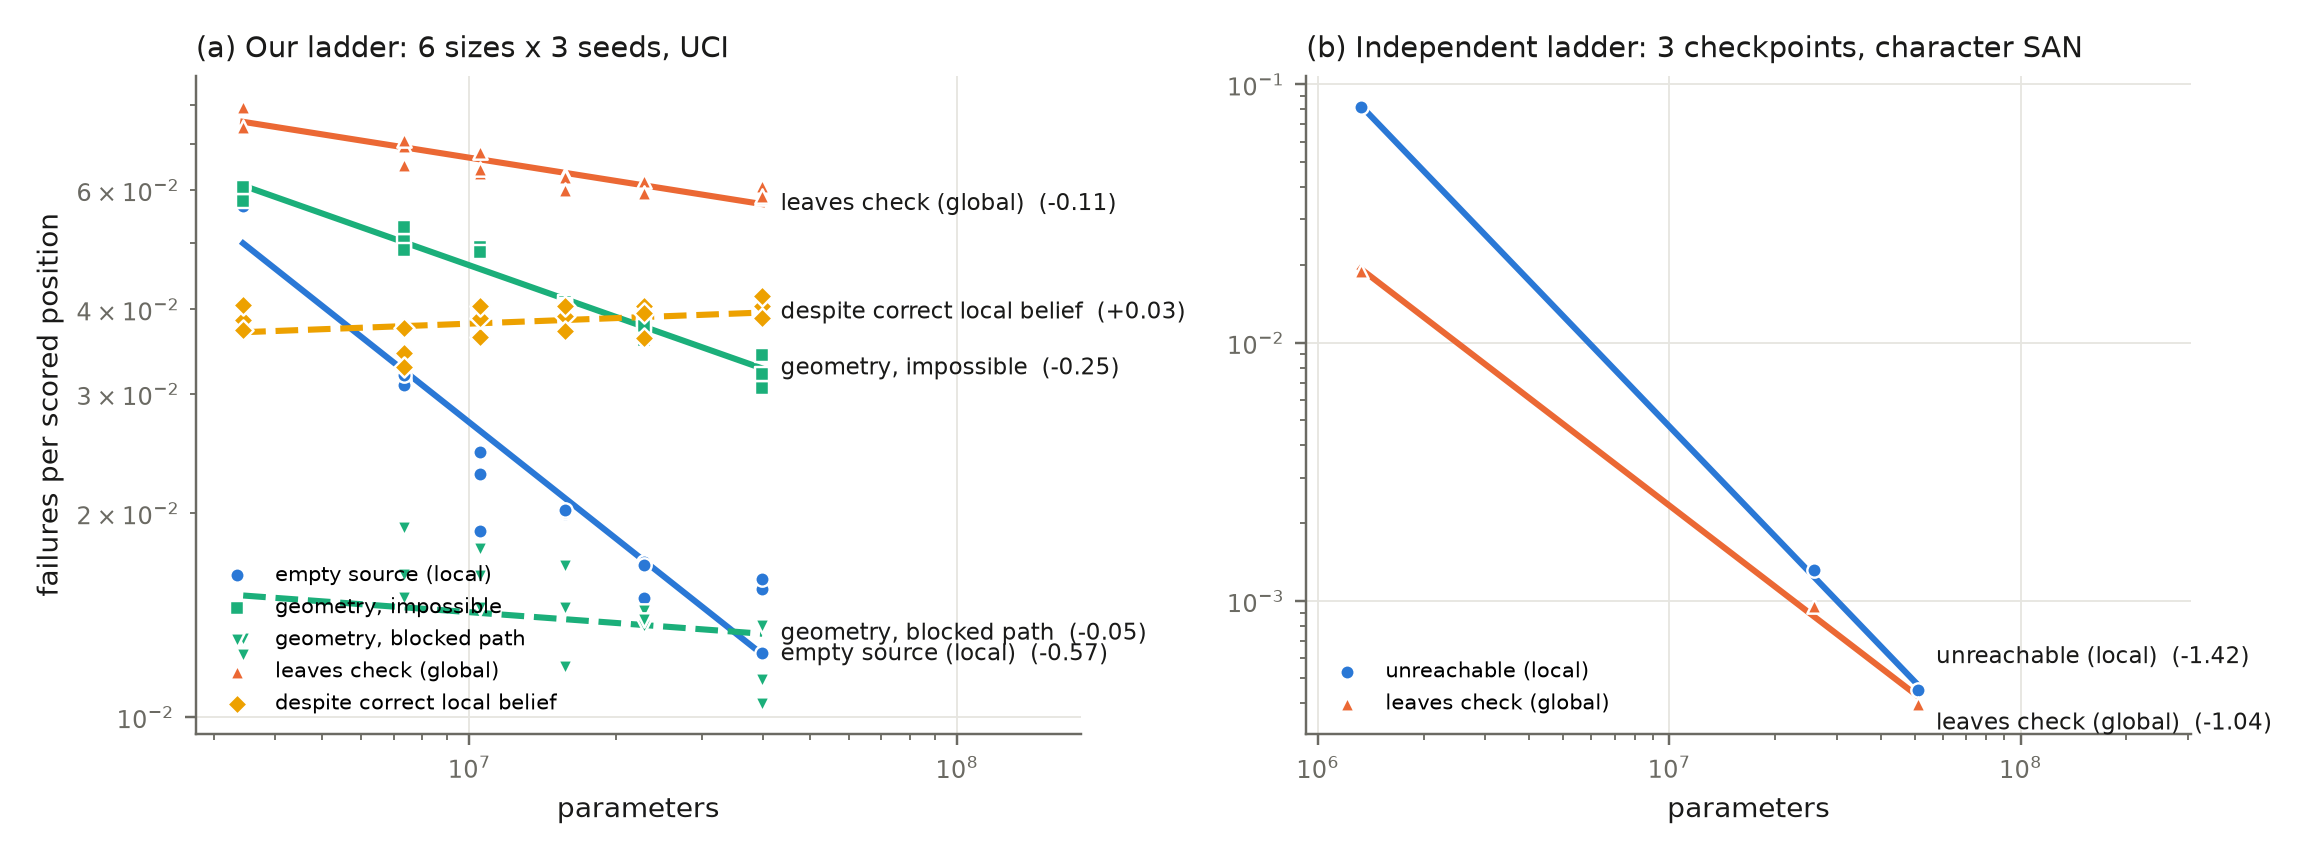
\includegraphics[width=\linewidth]{scaling.png}
\caption{Absolute failure rate against parameter count, log-log, so each line is a
power law and its slope, shown in each label, is the exponent. (a) Our ladder; each
point is one run. (b) An independent character-level ladder
(Section~\ref{sec:external}); each point is one checkpoint. In both, the local
class falls faster than the global one.}
\label{fig:scaling}
\end{figure}

Every class falls with size, so the result is not that larger models get worse at
anything. It is that they get better at different things at very different rates
(Table~\ref{tab:exponents}, Figure~\ref{fig:scaling}a). The extremes order
themselves by how local the rule is, but the ordering is not monotone across every
class and we do not claim it is. Castling improves faster than impossible movement,
at \result{rgExpCastle} against \result{rgExpGeomImp}, despite needing more than the move's two squares;
and blocked paths, which need only one further square, have the shallowest point
estimate of any class, \result{rgExpGeomBlk}, shallower even than check violations. Both
intervals exclude zero, so these are differences in rate rather than one class failing
to improve. What the data support is the specific
comparison. Errors decidable from the move's own two squares, pooled, fall with
exponent \result{rgExpLocalPooled} [\result{rgExpLoLocalPooled}, \result{rgExpHiLocalPooled}], against
\result{rgExpCheck} for check violations, a paired differential of \result{rgDiffCheckLocal}
[\result{rgDiffLoCheckLocal}, \result{rgDiffHiCheckLocal}]. Taken singly, empty-source errors fall with exponent
\result{rgExpEmpty}; geometry splits into movements no arrangement of the other squares
would permit, with \result{rgExpGeomImp}, and blocked paths, which do depend on the squares
between source and destination, with \result{rgExpGeomBlk}; and check violations, which
depend on every attacker's position, with \result{rgExpCheck}. The paired differential
between the check and empty-source exponents is \result{rgDiffCheckEmpty}
[\result{rgDiffLoCheckEmpty}, \result{rgDiffHiCheckEmpty}], and it excludes zero.

This is a claim about composition, and composition shifts accordingly. The
empty-source share of illegal moves falls from \result{rgShareEmptyFirst} to
\result{rgShareEmptyLast} while the check share rises from \result{rgShareCheckFirst} to
\result{rgShareCheckLast}; geometry taken together moves only from \result{rgShareGeomFirst} to
\result{rgShareGeomLast}, its impossible part barely at all, from \result{rgShareGeomImpFirst}
to \result{rgShareGeomImpLast}. The shift is
substantially one class collapsing into another rather than diffuse rebalancing.
Within models, check violations also concentrate at depth: their share rises from
early to late game in \result{rgDepthRises} of \result{nRungs} rungs, from
\result{rgDepthEarly} to \result{rgDepthLate} at the largest.

Nothing in this section uses model internals. The measurement is a rules engine
and a move counter, which makes it reproducible against any chess model and immune
to objections about probe validity.

\paragraph{Why we do not extrapolate the fitted lines.}
The obvious next step is to extend the fitted lines beyond our largest model and
report what they imply at, say, one billion parameters. We did this in an earlier
version of this analysis and it is wrong, for a reason that applies to any
per-category scaling fit and that we have not seen stated.

The categories partition the illegal moves. Their absolute rates must therefore sum
to the illegal-move rate at every scale. The difficulty is not that approximate
in-range fits disagree slightly, which is ordinary and harmless; several curves can
each describe the data well over a range without any contradiction. It appears when
those fits are treated as jointly exact and extended, because then the identity is
being asserted at scales where the functional forms cannot satisfy it. The \result{rgNClasses} independently fitted
power laws of the corrected partition, with \result{rgNClasses} different exponents, cannot
satisfy that identity away from the fitted
range: the shallowest exponent must eventually dominate a total that is itself
falling faster. The failure is not gradual. Summing the independently fitted parts
and dividing by the independently fitted whole gives \result{cmpOverLarge} at our
largest rung, which is fit noise, but \result{cmpOverBn} at one billion parameters
[\result{cmpOverBnLo}, \result{cmpOverBnHi}, above one in
\result{cmpOverBnFrac}\% of resamples] and \result{cmpOverTn} at one trillion.
Parts holding nearly three times the whole is not a wide estimate, it is an
arithmetic impossibility, and it means the extrapolation was never reporting the
exponents' implications at all. It is worth noting that the violation runs in the
direction that flatters our argument, since the categories we claim survive are
exactly the shallow ones that grow without bound.

\paragraph{A closed compositional fit.}
The repair is to fit the composition on the simplex rather than one category at a
time. The simplest repair is to stop fitting the aggregate and define it as the sum
of the categories, which satisfies the identity at every scale and keeps every
category exponent. Dividing through, the implied shares are a softmax linear in
$\log N$, so the compositional form and the derived total are the same model and
not a further choice. What the repair costs is the aggregate exponent: the derived
total is not a power law, and its effective slope drifts with scale. Coherence is not bought with fit quality. In range the closed model
attains RMSE \result{cmpRmseSimplex} across the \result{nRuns} runs against
\result{cmpRmseIndep} for the uncoupled fits, so it is at least as good on the
data while being the only one of the two that can be extended.

Under the closed model the check category's share rises across the range we are
willing to project, from \result{cmpCheckLarge} at our largest rung, while the locally
decidable categories decline. It does not rise to one, and here the corrected
partition changes the picture rather than merely refining it. Whichever category has
the shallowest exponent must eventually take the whole share, and before geometry was
split that category was the check class. It is now blocked paths, at \result{cmpAstar}
against the check class's \result{rgExpCheck}. The two are close enough that the crossing
falls outside the range we project at all: the check share rises monotonically to
\result{cmpCheckMax} across it, and blocked paths overtake it only further out. The paper's
qualitative claim about the observed range is unchanged, and the trajectory is now
bounded by construction rather than unbounded as in the earlier projection.

We put little weight on that asymptotic reordering, and say so here rather than
letting the appendix imply otherwise. It is decided entirely by the blocked-path
exponent. On the full set that exponent is \result{rgExpGeomBlk} [\result{rgExpLoGeomBlk},
\result{rgExpHiGeomBlk}], separated from the check class's \result{rgExpCheck} by less than the width
of either interval. Which of the two is shallower decides the entire asymptotic
story, and the data do not resolve it. The claim we defend is the ordering in range; which class wins at
scales far beyond the data is determined by the least well measured number we have.

We no longer report projected class shares at specific far-off scales in the main
text. The overspend ratios above are at those scales and stay, because what they
demonstrate is an inconsistency in a fitting procedure rather than a prediction about
models: the point is precisely that those numbers cannot be what the fits imply.
Enforcing
arithmetic consistency removes one objection to extrapolating, that the parts and the
total contradicted each other, but it does not supply a licence to extend a fitted
exponent far past the data, and we have independent reason here not to: the check
class shows detectable curvature inside the observed range (Section~\ref{sec:limits}),
so the in-range slope is already not a constant. The projected values are given in
Appendix~\ref{app:proj} for readers who want them, as an illustration of the closed
model's shape rather than as a prediction.

The same discipline applies to the failure share despite correct local decoding,
the fraction of illegal moves
occurring despite correctly decoded local belief. It is not a member of the
partition, since it cuts across the classes, but it is a proportion, and fitting a
proportion linearly in $\log N$ is unbounded in exactly the same way. Fitted on the
logit it increases with size from \result{cmpPolicyLarge} at our largest rung, having been
observed between \result{cmpPolicyObsLo} and \result{cmpPolicyObsHi}, and remains bounded above
by one however far it is extended; the projected values are in
Appendix~\ref{app:proj}. We report
it separately rather than folding it into the simplex; an earlier version of this
analysis did fold it in, which is wrong and which manufactured a spurious interior
maximum in the check category.

\paragraph{The failure is forced, not particular to us.}
Let the parts have exponents $a_i$ and the total exponent $b$, and let
$a^\star=\max_i a_i$. The sum of the parts is asymptotically $N^{a^\star}$ and the
total is $N^{b}$, so the ratio grows like $N^{a^\star-b}$ and diverges precisely
when $a^\star>b$. This is not a coincidence to be checked case by case. Fitted in
range, $b$ tracks the rate-weighted mean of the $a_i$, and a maximum is at least a
weighted mean, with equality only if every exponent is identical. Our own values
make the point: $a^\star$ is \result{cmpAstar}, attained by the \result{cmpAstarClass} class,
the weighted mean is
\result{cmpWeighted}, and the separately fitted $b$ is \result{cmpBtotal}, giving
divergence \result{cmpDiverge}.

The claim this supports needs stating carefully, because a stronger version does not
follow. Divergence requires $a^\star > b$, and nothing forces that for an arbitrary
$b$; a total assigned a sufficiently shallow exponent by hand would not diverge. What
makes the inconsistency generic is how $b$ is obtained in practice. An aggregate
fitted over the same range as the parts tracks their rate-weighted mean, which lies at
or below the maximum and equals it only when every exponent is identical, so
$a^\star > b$ holds whenever the exponents genuinely differ. The underlying
mathematical point is simpler and does not depend on the fitting procedure at all: a
sum of positive power laws with differing exponents does not itself have a constant
power-law exponent, so an exact total and a single fitted exponent for it are
different objects. Reporting both is what creates the contradiction, and the
resolution is to derive the total rather than fit it. For our own numbers the scale at
which the two descriptions part company is computable from
the reported exponents and coefficients together, since where the curves cross depends
on their intercepts as well as their slopes: ours passes a ten percent overspend at
\result{cmpBreakdown} parameters, well below the billion the earlier projection
used.

We checked this on a model family we did not train. Refitting Karvonen's ladder
over its own \result{cmpExtNclass} classes gives divergence \result{cmpExtDiverge},
an overspend of \result{cmpExtOverBn} at one billion parameters, and a breakdown
scale of \result{cmpExtBreakdown}. A different tokenisation, a different taxonomy,
a different training set and a different laboratory reproduce the defect at the
same order of magnitude, which is what the argument above predicts and what makes
us report it as a property of the method rather than of our data.

% ====================================================================
\section{External Validity}
\label{sec:external}

\paragraph{An independent ladder.}
Karvonen's lichess checkpoints \citep{karvonen2024emergent} differ from ours in
every respect we could change without training: character-level PGN rather than
one token per move, standard algebraic notation rather than UCI, roughly 16M
training games rather than ours, and different training code. We use its
\result{kParamsSix}, \result{kParamsEight}, and \result{kParamsSixteen} checkpoints
and read the model's move by greedy character decoding at move boundaries.

\paragraph{Verifying the adapters.}
Every step between an external model and our measurements fails silently rather
than with an error: a wrong vocabulary, a misaligned board, or a missed weight
transpose all yield plausible output. Each was therefore checked before use and
the checks rerun and recorded. The released weights ship without a tokenizer, so
the \result{acVocab}-character vocabulary was reconstructed and accepted only after
the model continued \result{acOpenLegal} of \result{acOpenTotal} standard openings
legally. Board state was aligned to the character before each move and verified
three ways at \result{acAlignSites} sites, by independent replay, by re-parsing
the text prefix, and by the boundary character, with \result{acAlignProblems}
disagreements. Checkpoints stored in a different weight layout were converted, and
\result{acAllNano} trained checkpoints then played \result{acNanoLegal} of
\result{acNanoTotal} moves legally from the opening, while the randomly initialised
control failed at its first move, as it should. A cached decoder used for speed
matched the uncached one at all \result{acCacheSites} sites tested, the
algebraic-notation classifier passed \result{acSanCorrect} of \result{acSanCases}
hand-written cases, and our OthelloGPT forward pass chose a legal move at
\result{acOthLegal} of \result{acOthTotal} positions.

Algebraic notation changes the taxonomy in an instructive way. It never names a
source square, so the empty-source class cannot occur: a model that does not name
the square cannot place a piece on an empty one. The nearest local class is
\emph{unreachable}, no piece of the named type can reach the destination, which
also absorbs path blocking. That makes the local class less local than ours and
biases the comparison against the result.

The ordering holds (Table~\ref{tab:external}, Figure~\ref{fig:scaling}b).
Unreachable errors fall with exponent \result{kExpUnr} and check violations with
\result{kExpLc}, a differential of \result{kDiff}, against \result{rgDiffCheckEmpty} on
our ladder. The local share of failures falls from \result{kShareUnrSix} to
\result{kShareUnrSixteen} while the check share rises from \result{kShareLcSix} to
\result{kShareLcSixteen}. Within the smallest checkpoint the check share rises from
\result{kSixLcEarly} to \result{kSixLcLate} across depth while the unreachable
share falls from \result{kSixUnrEarly} to \result{kSixUnrLate}. At comparable size
this ladder fails far less often than ours, because it was trained on far more
data, so only exponents are comparable and never levels.

\begin{table}[t]
\centering\small
\caption{Independent ladder. Absolute rates per scored position. With three
checkpoints the uncertainty in the fit itself is poorly determined, and the intervals
propagate only each checkpoint's sampling noise in class shares, so they are a lower
bound on uncertainty rather than a confidence statement about the slope. Deleting
each checkpoint in turn leaves three two-point fits whose differential spans
[\result{extLooMin}, \result{extLooMax}], same sign throughout; we report that spread in place of an
interval we cannot honestly construct.}
\label{tab:external}
\begin{tabular}{lcccc}
\toprule
checkpoint & illegal & failures & unreachable & leaves check \\
\midrule
\result{kParamsSix}     & \result{kIllSix}     & \result{kFailSix}     & \result{kAbsUnrSix}     & \result{kAbsLcSix} \\
\result{kParamsEight}   & \result{kIllEight}   & \result{kFailEight}   & \result{kAbsUnrEight}   & \result{kAbsLcEight} \\
\result{kParamsSixteen} & \result{kIllSixteen} & \result{kFailSixteen} & \result{kAbsUnrSixteen} & \result{kAbsLcSixteen} \\
\midrule
exponent & & & \result{kExpUnr} [\result{kExpUnrLo}, \result{kExpUnrHi}] & \result{kExpLc} [\result{kExpLcLo}, \result{kExpLcHi}] \\
\bottomrule
\end{tabular}
\end{table}

\paragraph{A game with non-local rules.}
Othello legality is non-local by construction: a move is legal only if it flanks a
line of opponent discs, so it is never decidable from the target square. There is
no published Othello ladder, so no exponent can be fitted, and we test only what
the claim implies for a single well-trained model: that its residual failures
should be the non-local kind. In Li's synthetic OthelloGPT \citep{li2023emergent},
across \result{othPos} positions and \result{othFail} failures, \result{othOccupied} are moves onto an
occupied square and \result{othNoFlank} are moves that flank nothing. The remaining
\result{othPass} is a pass token emitted where passing was not available, which is neither
kind; we count it rather than round it away, which is why the non-local share is
\result{othNoFlank} of \result{othFail} and not all of them. The comparison is weaker than it looks, because discs never leave a
square: whether a square is occupied reduces to whether it appears in the move
history, which requires no state tracking at all. Failures also concentrate late,
\result{othDepthA}, \result{othDepthB}, and \result{othDepthC} across the three move
bands.

\paragraph{Heavy training.}
The mechanism in Section~\ref{sec:mech} rests on three measurements taken on
models trained on about a hundred thousand games. We repeated all three on
Karvonen's character-level model trained on roughly 16M games
(Table~\ref{tab:chessgpt}). Its board state at depth is better than ours, so the
comparison is not against a model whose state was hard to extract: probe accuracy
on occupied squares is \result{cgProbeFirst} early and \result{cgProbeLast} late,
against \result{ourProbeFirst} and \result{ourProbeLast} for ours. Human games give
only \result{cgNIllH} illegal moves, so we also report uniformly random legal play,
which lifts the illegal rate from \result{cgIllH} to \result{cgIllR}.

\begin{table}[t]
\centering\small
\caption{The three mechanism measurements on a model trained on roughly 16M games.
Belief consistency is the fraction of illegal moves legal on the probe-decoded
board. The AUC on our models is a mean over depth buckets and on Chess-GPT is
pooled over depth, which is not the same quantity; only the sign and rough size of
the move-touched advantage are compared. Chess-GPT's move-touched square is the
destination, since algebraic notation names no source.}
\label{tab:chessgpt}
\begin{tabular}{lccc}
\toprule
& ours & Chess-GPT, human & Chess-GPT, random play \\
\midrule
belief consistency, own board & \result{ourBelOwn} & \result{cgBelOwnH} & \result{cgBelOwnR} \\
\quad mismatched board        & \result{ourBelMis} & \result{cgBelMisH} & \result{cgBelMisR} \\
\quad random move             & \result{ourBelRand} & \result{cgBelRandH} & \result{cgBelRandR} \\
\quad own / mismatched        & \result{ourBelRatio} & \result{cgBelRatioH} & \result{cgBelRatioR} \\
\midrule
AUC, whole board              & \result{ourAucAgg} & \result{cgAucAggH} & \result{cgAucAggR} \\
AUC, move-touched             & \result{ourAucAct} & \result{cgAucActH} & \result{cgAucActR} \\
\quad advantage               & \result{ourAucDiff} & \result{cgAucDiffH} & \result{cgAucDiffR} \\
\midrule
edit, state direction         & n/a & \result{cgEditH} & \result{cgEditR} \\
edit, norm-matched random     & & \result{cgEditRandH} & \result{cgEditRandR} \\
edit, manipulation check      & & \result{cgFlipH} & \result{cgFlipR} \\
\bottomrule
\end{tabular}
\end{table}

All three hold, at reduced size. The model's illegal moves are legal on its own
decoded board far more often than on another position's, at a ratio of
\result{cgBelRatioR} against \result{ourBelRatio} for ours. Fidelity at the square
the move targets predicts illegality where whole-board fidelity is near chance.
And emptying a square in the model's belief lowers the probability of moves from
it, by \result{cgEditDiffR} [\result{cgEditDiffRLo}, \result{cgEditDiffRHi}] beyond a
norm-matched random edit, with the decoded square flipped in \result{cgFlipR} of
cases. Heavy training weakens coherent error without removing it.

% ====================================================================
\section{Mechanism}
\label{sec:mech}

Why does scale leave the global class behind? Three measurements, using the probe
and edit instruments of \priort, point to the same answer.

\paragraph{Coupling is local.}
We repair the model's belief at the squares its illegal move touches by adding
probe-derived occupancy directions to the residual stream, and score the change in
a forced-choice preference $r = P(m^\ast)/(P(m^\ast)+P(m_{\mathrm{ill}}))$ between
the best legal move and the illegal one. The ratio cancels the softmax normalising
constant, so it is unaffected by a uniform rescaling of all probabilities, but it is
not invariant to temperature: $r_T = \sigma((z_{m^\ast} - z_{m_{\mathrm{ill}}})/T)$ moves
toward one half as $T$ rises. We state this because an earlier version claimed
invariance to flattening in general, which is wrong, and because temperature alone
cannot explain the disagreement between metrics reported below: rescaling logits
does not reorder them, so it cannot change which move is top-1. An edit that
produces more legal top-1 moves must be reordering logits, not merely flattening
them, and distinguishing the two needs a temperature-only control. We report that
control in Section~\ref{sec:inversion}: top-1 legality turns out to be exactly
invariant to temperature, so flattening is ruled out as the explanation. Two controls
matter here as well. A wrong-target edit installs the same
occupancy at an unrelated square; an irrelevant edit spends an identical budget on
squares that are wrongly decoded but not touched by the move. Both are matched to
correct repair in magnitude and construction, and all contrasts are taken on
positions where the two edits changed the output entropy comparably. Across
\result{metaKillN} models, correct repair beats wrong-target in
\result{metaKillPos} (sign test \result{metaKillP}) and beats the irrelevant edit in
\result{metaLocPos} (\result{metaLocP}), mean advantage \result{metaLocMean}. Only
\result{metaLocSig} of the irrelevant-edit contrasts exclude zero individually,
because matching retains about half the positions per run; the evidence is that
none of \result{metaLocN} is negative. Correcting the squares the move depends on
changes behaviour more than correcting other wrong squares, which reconciles a
weak whole-board coupling \citep{balogh2026verification} with a strong local one.

\paragraph{Correction reaches about two squares.}
The repair channel works: when we corrupt a single square ourselves and repair it,
the model recovers a legal move in \result{indRec} [\result{indRecLo},
\result{indRecHi}] of cases against \result{indRand} for a random repair. On the
model's own failures, repair at the touched squares restores a legal move in only
\result{natRepaired}, a \result{indNatRatio}-fold gap. Natural failures involve a
median of \result{natDivMedian} wrongly decoded squares, so we tried repairing all
of them. It fails in a specific way (Table~\ref{tab:mechanism}): a two-square edit
restores the decoded value at \result{fidTargetTwo} of its targets, while an
all-square edit restores \result{fidTargetAll}, and full strength per square does
no better at \result{fidTargetPerSq}. Whole-board repair lowers occupied-square
decoding accuracy from \result{fidOccBefore} to \result{fidOccAfter}. The instrument
succeeds more reliably on small corrections and does not install a reliable
whole-board correction at any magnitude we tested. We tested two sizes, two squares
and all divergent squares, so this bounds the procedure at those two points and is
not a capacity curve; establishing one would need intermediate edit sizes at matched
target difficulty and a stated rule for choosing edit strength.

\begin{table}[t]
\centering\small
\caption{Mechanism summary. Meta rows count models out of \result{metaKillN};
repair and fidelity rows are from a single model.}
\label{tab:mechanism}
\begin{tabular}{lc}
\toprule
correct beats wrong-target edit, models          & \result{metaKillPos} / \result{metaKillN} \\
correct beats irrelevant-square edit, models     & \result{metaLocPos} / \result{metaLocN} \\
\midrule
induced single-square corruption, recovered      & \result{indRec} \\
\quad random repair                               & \result{indRand} \\
natural failures, recovered by touched-square repair & \result{natRepaired} \\
\midrule
decoded value restored, two-square edit          & \result{fidTargetTwo} \\
decoded value restored, all-square edit          & \result{fidTargetAll} \\
occupied-square accuracy, before and after all-square edit & \result{fidOccBefore} to \result{fidOccAfter} \\
\bottomrule
\end{tabular}
\end{table}

\paragraph{What the tested correction does not reach.}
Where decoded belief is already correct at both squares a move touches, a check
violation accounts for \result{rgPolCheck} of failures on average against
\result{rgPolGeom} for geometry taken together, and is the largest class in
\result{rgPolLargest} of \result{rgPolModels} models. Such failures cannot be attributed
to the decoded belief being wrong at the move's squares. Their absolute rate is
flat with size, exponent \result{rgExpCorrLoc} [\result{rgExpLoCorrLoc}, \result{rgExpHiCorrLoc}], a differential
against empty-source errors of \result{rgDiffCorrLocEmpty} [\result{rgDiffLoCorrLocEmpty},
\result{rgDiffHiCorrLocEmpty}], on the same paired bootstrap as the others.

\paragraph{The flat rate is two effects cancelling, not one effect absent.}
An earlier version of this paper read that flat exponent as the underlying failure
propensity being untouched by scale. It does not support that, and the quantity is
a joint event:

\begin{equation*}
P(\text{illegal} \\ \text{correct local decoding}) = P(\text{correct local decoding}) \cdot P(\text{illegal} \mid \text{correct local decoding}).
\end{equation*}

Both factors move. Across the \result{jcRuns} runs the marginal rises with exponent
\result{jcMarg} [\result{jcMargLo}, \result{jcMargHi}], decoding accuracy going from \result{jcMargFirst} to \result{jcMargLast},
and the conditional falls with exponent \result{jcCond} [\result{jcCondLo}, \result{jcCondHi}], whose interval
excludes zero. The joint rate is flat because the two nearly cancel. The
decomposition is exact rather than estimated, so this is a restatement of the same
number and not a competing measurement.

Calling it exact commits us to something checkable, and it is worth saying what.
Because the identity holds position by position, the logs add, and an ordinary
least-squares slope is a linear functional of the response, the three exponents
must sum exactly when all three are fitted on the same runs with the same
predictor. They do, to \result{jvAddErr}: the marginal and conditional exponents
add to the joint exponent of Table~\ref{tab:exponents} and not merely to something
close to it. An earlier version of this paper failed that check, because the joint
rate was taken from the superseded classification pass while the two factors came
from the corrected one. Two numbers that must add are a cheap and unforgiving test
of whether a decomposition has been assembled from one pass or two.

The correct reading is therefore the opposite of the one we drew: scale does reduce
the rate at which a model fails while holding correct local state, and the flat
joint rate conceals it because a better model decodes correctly more often and so
has more occasions on which to fail that way. What survives is the weaker claim
that this component declines more slowly than the locally decidable classes, which
is what the differential measures.
An earlier oracle-free attempt to repair state by re-presenting information the
model already attends to also failed, leaving the late-game illegal rate at
\result{refreshRepair} against \result{refreshNoop} without intervention.

We do not claim these failures are unrepairable in principle. The instrument cannot
install a multi-square correction, so whether the residual is genuine policy
failure or simply beyond its reach is undetermined, and we recorded the stronger
reading as retracted (Appendix~\ref{app:integrity}). The claim is narrower and
sufficient: the component scale leaves behind is concentrated in exactly the
failures that the correction procedure we tested, applied at the move's squares,
does not address. Whether some other local intervention could reach them is open.

% ====================================================================
\section{Intervention Metrics Rank Repairs Differently}
\label{sec:inversion}

Interventions on state are usually scored by whether the model's output becomes
legal. On our repair edits that metric orders the conditions nearly in reverse
(Table~\ref{tab:inversion}). On one model, correct repair produces the largest
preference shift, \result{drCorrect}, and a random direction the smallest,
\result{drRand}; yet after the edit the random direction leaves a legal top-1 move
in \result{nlRand} of cases and correct repair in \result{nlCorrect}. The random
direction also raises output entropy most, by \result{dentRand}. The tempting reading is
that this is hedging, moving probability off a confidently illegal move and onto
whatever else is plausible. That reading does not survive the temperature control
below: flattening a distribution cannot change which move ranks first, so raised
entropy cannot by itself be what produces the extra legal top-1 moves. The entropy
change is real and is reported; the mechanism behind the ranking change is not
established here.

\begin{table}[t]
\centering\small
\caption{Repair conditions on one model (\result{repN} positions, \result{repGames}
games): change in forced-choice preference, fraction of top-1 moves legal after
the edit, change in entropy, and how often the target square's decoded value
flipped. The null edit re-installs values already decoded correctly and is zero by
construction.}
\label{tab:inversion}
\begin{tabular}{lcccc}
\toprule
condition & $\Delta r$ & legal after edit & $\Delta$ entropy & decode flipped \\
\midrule
correct repair   & \result{drCorrect} & \result{nlCorrect} & \result{dentCorrect} & \result{flipCorrect} \\
irrelevant squares & \result{drIrr}   & \result{nlIrr}     & \result{dentIrr}     & \result{flipIrr} \\
wrong target     & \result{drWrong}   & \result{nlWrong}   & \result{dentWrong}   & \result{flipWrong} \\
random direction & \result{drRand}    & \result{nlRand}    & \result{dentRand}    & \result{flipRand} \\
null             & \result{drNull}    & \result{nlNull}    & \result{dentNull}    & \result{flipNull} \\
\bottomrule
\end{tabular}
\end{table}

This is not one model. In \result{invCount} of \result{invN} models the random
direction produces more legal moves than correct repair while correct repair
produces the larger preference shift (sign test \result{invP}), and the random
direction has the best legal-move rate of all four edits in \result{invRandBest} of
them.
Its advantage in legal moves over correct repair ranges from \result{invGapMin} to
\result{invGapMax}.

The same artefact affects our own preference metric if uncontrolled. The raw
advantage of correct repair over wrong-target is \result{rawCW}; restricted to
positions where both edits changed entropy comparably it is \result{matchedCW}
[\result{matchedCWLo}, \result{matchedCWHi}], \result{inflation} times smaller. The
edit also responds gradedly to strength: preference rises from \result{sweepQ} at a
quarter of calibrated strength to \result{sweepOne} at calibrated strength, then
turns to \result{sweepTwo} and \result{sweepFour} at double and quadruple, a
rise-then-collapse that is harder to explain as generic damage than a monotone
decline would be.
Studies that score state interventions by illegal-move rate, or by any error rate
a flatter distribution can lower, need not be measuring what it is taken to measure.
We do not claim the mechanism is distributional flattening: temperature alone cannot
reorder logits and so cannot change which move is top-1, and the random edits do
change it, so something other than flattening is at work and we have not identified
it.

% ====================================================================

\paragraph{A temperature-only control, which rules out the flattening account.}
An earlier version of this paper explained the inversion by saying that illegal-move
rate rewards edits which flatten the output distribution. That account cannot be
right, and the reason is short enough to settle without an experiment: dividing
logits by a temperature is a monotone transformation, so it cannot reorder them, so it
cannot change which move ranks first. Top-1 legality is therefore invariant to
flattening exactly, not approximately, and whatever the random edits are doing, they
are not winning on this metric by hedging.

We ran the control regardless, because an assertion of exact invariance is a claim
about our implementation as well as about the mathematics, and because the quantities
that are not invariant are the informative part. Over \result{tcPos} scored positions
of the largest model, sweeping temperature across a \result{tcFold}-fold range from
\result{tcTmin} to \result{tcTmax} leaves top-1 legality at \result{tcTop1} throughout, with a maximum
deviation of \result{tcTop1Dev}: not small but identically zero, as it must be. The ranks of
the fixed candidate pair do not move either.

The other two measures move a great deal. Total probability mass on legal moves falls
from \result{tcMassHi} to \result{tcMassLo} over the same sweep, a factor of \result{tcMassFold}, and the
forced-choice preference between the best legal move and the top illegal one drifts
from \result{tcPrefHi} toward \result{tcPrefLo}, approaching the indifference value of one half as
the temperature rises. The candidate pair is fixed from the unmodified logits before
the sweep, so this is the preference moving and not the selection of what to compare.

Three measures of the same model under the same manipulation therefore behave in three
ways: one cannot move at all, one collapses, and one decays toward indifference. This
is the defensible form of the paper's point about measurement. It is not that
illegal-move rate is an inverted measure of quality, nor that the random edits are
merely hedging. It is that the random edits genuinely do better on top-1 legality,
the repair genuinely does better on the forced choice, and these cannot both be
summarised by one number. Which of them tracks move quality is a question this paper
does not answer, and identifying what the random edits change about the ranking, given
that flattening cannot, is the obvious next experiment.

\section{Discussion}

The practical content is about where effort goes. The class that falls most slowly
with size is the one defined by constraints spanning the whole board, and on our
evidence it is also the class that correcting the model's belief about a move's own
squares does not reach. It does fall: its exponent is \result{rgExpCheck} with an interval
excluding zero. The quantity that is close to flat is a different one, the joint rate
of failures occurring despite correct local decoding, and that flatness is itself two
effects cancelling. We read this, as an interpretation we have not tested
directly, as a caution for interventions such as auxiliary board losses and state
supervision: they aim at the model's knowledge of where pieces stand, and the
failures most directly attributable to that knowledge are the ones scale is already
removing. An intervention that lowers total error while leaving the global class
flat may have improved only what scale improves anyway, and should be evaluated by
its effect on that class.

This also bounds what an intervention study can show. A training comparison that
targets state-attributable failure is adequately powered on our data, detecting a
change of \result{powMdePct}\% of that component with seed variation contributing
little (relative spread \result{powSeedRel}), but the component is a small share of
what goes wrong, so a detectable improvement is a small behavioural one.

A methodological point generalises further than our subject. Whenever failures are
decomposed into categories and each category is given its own scaling exponent, the
fits sit alongside a separately fitted aggregate, the two make claims that cannot
both hold, and extrapolation is where the conflict becomes visible. The check costs nothing: sum the extrapolated parts and see whether they
still make the whole. We report it because our own uncoupled fits passed every gate
in this paper, agreed with the data in range, and were still projecting an
impossibility two orders of magnitude out. Any decomposition of error into
categories that scale at different rates, whether by capability, benchmark subset,
or error type, has this property, and fitting on the simplex removes it without
costing accuracy. We supply the check as \texttt{code/closure\_check.py}, which
needs only the exponents and intercepts such papers already print.

One consequence is easy to miss, and we missed it. An inadmissible fit voids
negative conclusions as well as positive ones. While preparing this section we
tested whether failure composition is governed by achieved competence rather than
by size, rejected it because the fitted shares exceeded one, and recorded it as
refuted. That rejection was worthless: predicting an impossibility is what the
uncoupled form does everywhere, so its disagreement with data carries no evidence
about the hypothesis under test. Refitting the same comparison on the simplex, in
competence coordinates, and predicting Karvonen's checkpoints out of sample does
refute it, by a total variation distance of \result{cmpCompTV} against
\result{cmpSizeTV} for size coordinates and \result{cmpBaseTV} for predicting our
own mean composition. The conclusion survived; the first argument for it did not.
A model that cannot make an admissible prediction cannot be used to reject
anything.

The local and global distinction is not specific to chess. Wherever a checker can
say not only that a step is wrong but which constraint it violated, program
execution, spreadsheet recalculation, and formal proof among them, the same
decomposition is available, and the question of which violations scale removes can
be asked without any access to model internals.

% ====================================================================
\section{Implications for Individuals, Organisations, and Society}
\label{sec:implications}

\paragraph{For the people on the receiving end of a long-horizon failure.}
The errors this paper separates are not equally visible to the person affected. An
error decidable from the move's own squares is the kind a user can usually catch:
it contradicts something in front of them. An error that is locally consistent and
globally wrong is not, because every part of it looks right. Our measurements say
scale removes the first kind several times faster than the second, so the errors
that survive in larger systems are disproportionately the ones a non-expert cannot
see. That shifts the burden of catching mistakes from the person who can check a
detail to the person who can check the whole, and in most deployments those are not
the same person and the second is not present.

\paragraph{For managers and organisations.}
The practical reading is about where a mitigation budget goes. A class of failure
that scale removes on its own is a poor target for engineering effort, and a class
with an exponent near zero will still be there after the next model upgrade. Our
estimate is that errors surviving a correct local belief have a flat joint rate,
exponent \result{rgExpCorrLoc}, which decomposes into a rising chance of decoding the
position correctly and a conditional failure rate falling with exponent \result{jcCond}.
The improvement in the conditional rate is real but is cancelled in the headline
number, so an
organisation reading only the joint rate will conclude wrongly that scale does nothing
for this class. We do not read the conditional decline as a measurement of planning
ability: correct decoding at two squares is not a correct global state, and the group
being conditioned on changes composition across models, so this is a conditional
association rather than an isolated capability.
An organisation deciding between waiting for the next generation and funding a
mitigation can, in a domain with a checker, measure which class its own failures
fall into rather than arguing about it. The second lesson is about measurement:
illegal-move rate, the metric most readily available, ranks a norm-matched random
edit above a correct repair in \result{invCount} of \result{invN} models, while the repair
produces the larger shift in a fixed forced choice. Two reasonable measures of the
same intervention disagree, so a single headline number cannot settle whether an
intervention helped.

\paragraph{Strategic implications.}
Treat the composition of failure, rather than its rate, as the quantity worth
tracking. A falling error rate is compatible with the dangerous share of errors
rising, and our ladder shows exactly that: the total falls while the fraction that
is globally rather than locally wrong increases. An organisation that reports only
the aggregate will see improvement in the period when its remaining failures are
becoming harder to detect. The capability to decompose is cheap where an oracle
exists and needs no access to model internals, so it is available to a buyer as well
as to a vendor, which matters when the two disagree about whether a known defect
will be fixed by scale.

\paragraph{For society and the public record.}
The decomposition used here needs a checker that can say not only that an output is
wrong but which constraint it violated. Chess has one for free. Program execution,
spreadsheet recalculation and formal proof have one too, and in those domains the
same question can be asked by anyone, at no cost, without the cooperation of whoever
built the system. Where no such checker exists, and most consequential deployments
are in that position, claims about which errors scale away cannot currently be
audited by anybody. We would rather state that plainly than let a result measured in
a game stand in for domains that cannot yet be measured.
% ====================================================================
\section{Limitations}
\label{sec:limits}

\begin{description}[nosep]
\item[Depth and width are confounded.] Both ladders grow depth and width together,
so an exponent in parameters does not isolate either.
\item[Three external checkpoints.] The independent ladder supports directional
agreement, not a second estimate of the slope; its intervals omit fit uncertainty.
\item[Notation changes the classes.] Algebraic notation removes the empty-source
class, and its nearest local analogue absorbs path blocking.
\item[Othello cannot test scaling.] No ladder exists, and its local class requires
no state tracking, so it is a consistency check rather than a replication.
\item[Consistency is not validation.] The derived total guarantees the
projection is arithmetically possible, which the uncoupled fits are not. It does
not make it observed: every scale past \result{paramsLarge} is extrapolation, and
a different link satisfying the same constraint would give different numbers while
agreeing that the uncoupled ones are inadmissible.
\item[The check class is not an exact power law.] Fitting it quadratically in
$\log N$ gives a curvature term whose bootstrap interval excludes zero, so the
exponent we report for it is a local slope over our range. This does not change its
sign, its separation from the local classes, or the ordering that is this paper's
result, all of which are about the fitted range. It does mean a reader should not
extend that one exponent far beyond the ladder.
\item[The residual is unattributed.] The repair instrument corrects about two
squares, so whether failures despite correct local belief reflect policy or
unreachable state is undetermined.
\item[Probe-based rows depend on a linear probe.] A nonlinear decoder of four times
the capacity gains only \result{capGapMin} to \result{capGapMax} across depth
(Appendix~\ref{app:capacity}), so decoder weakness does not explain decay, but the
probe-based rows inherit its approximation. The headline result uses no probe.
\item[One game family.] Chess and Othello both carry exact oracles, which is what
makes them measurable and what makes them unrepresentative of open-ended reasoning.
\end{description}

% ====================================================================

\paragraph{What the intervals cover, and the unit of variation.}
Intervals on the main ladder resample rungs, because seeds within a rung share an
architecture and are not independent draws of it. This makes the rung the unit of
variation and leaves within-run sampling noise over games and positions outside the
interval rather than inside it. We take rung-level variation to be the larger term,
but we have not decomposed the two, and a reader who wants a game-clustered interval
on a single run will not find one here. The external ladder differs: its per-
checkpoint class shares are bootstrapped clustering on games, so game-level noise is
propagated there and the fit uncertainty is what is missing instead.

The sign tests over the \result{nRuns} runs treat runs as exchangeable. Seeds within a rung
satisfy that by construction, differing only in initialisation and batch order.
Rungs do not: they differ systematically in size, which is the very thing under
study. A sign test pooled across rungs does not establish that an effect holds at every size
merely because the runs span sizes, and we separate the two statements. The observed
count is a description of these runs: the effect has the same sign in all of them.
The inferential claim a pooled sign test supports is the weaker one that the median
effect over this set of runs is nonzero. Neither licenses a statement about a model
drawn from some population of architectures, which \result{nRungs} sizes could not support.

\paragraph{Unequal scored sets in the external table.}
The external checkpoints were not all scored on the same number of positions. The
two larger ones share an identical set of \result{kPosLarge} positions, while the smallest was
scored on \result{kPosSmall}. The sets are nested rather than disjoint, the smaller being a
prefix of the same held-out corpus, so this is a difference in sample size and not
in sampling population. It still means the three rows of that table rest on unequal
precision, and the smallest checkpoint is also the one with by far the most failures,
so its shares are the best determined despite the smaller set. We also note that the
game count reported for each checkpoint is the number of games contributing at least
one failure, not the number scored, which is why it falls as the models improve.

\section{Conclusion}

Scale does not remove long-horizon errors evenly. In chess transformers it removes
errors decidable from a move's own squares several times faster than errors
decided by the whole board, the ordering replicates on an independent model family,
and the failures that occur despite correctly decoded belief at the move's squares
have a joint rate that is nearly flat, exponent \result{rgExpCorrLoc}, because a rising chance
of decoding the position correctly offsets a conditional failure rate that does fall,
exponent \result{jcCond}. The measurement needs only a rules engine. What it suggests is
that the failures worth studying at scale are the ones defined by global constraints,
and that interventions aimed at them should be judged on more than one measure, since
two reasonable scores of the same edit disagree and neither alone settles whether the
edit helped.

\section*{Declarations}

\paragraph{Disclosure statement.}
\ifanon Removed for double-anonymous peer review.
\else The authors report no conflict of interest. \fi

\paragraph{Funding.}
\ifanon Removed for double-anonymous peer review.
\else This research received no specific grant from any funding agency in the
public, commercial, or not-for-profit sectors. \fi

\paragraph{Data availability statement.}
\ifanon
The analysis code, every result file cited by the manuscript, and the macro
provenance record will be made available upon acceptance. External checkpoints are
public.
\else
The analysis code, every result file cited by the manuscript, and the macro
provenance record are available at
\url{https://github.com/MohitPratapSinghRathore/derived-total}. Trained checkpoints
are available from the corresponding author on reasonable request, being too large
to distribute with the repository. External checkpoints are public.
\fi

\paragraph{AI usage declaration.}
During the preparation of this manuscript the authors used a generative AI tool to
assist with language editing and refinement of the text, and with writing analysis
code. The authors reviewed and edited all output and take full responsibility for
the content of the paper. Generative AI was not used to generate or analyse the
study's data, which were produced entirely by the measurement pipeline described in
the paper.

\appendix

\section{Probe capacity}
\label{app:capacity}

Every fidelity curve in this line of work is read with a linear probe, which could
confound information leaving the representation with information becoming
nonlinearly encoded. On identical activations and budgets, a two-layer probe whose
hidden layer is four times the residual width improves occupied-square accuracy by
between
\result{capGapMin} and \result{capGapMax} across depth, with no tendency to widen.
The same nonlinear probe reaches \result{capCtlDeep} on a control task with
shuffled boards and \result{capRandDeep} on a randomly initialised model in the
deepest bucket, so there is no memorisation headroom for extra capacity to exploit.
Decay in these curves is therefore not explained by the weakness of a linear
decoder, though a single alternative decoder cannot rule out every nonlinear
encoding.

\section{Integrity record}
\label{app:integrity}

The analysis plan was frozen and hashed (SHA-256 prefix \texttt{\result{preregHash}}).
We state plainly what that does and does not establish, because an earlier version of
this statement claimed more than the record supports. A hash fixes a document's
content; it carries no time, so on its own it cannot show that the plan preceded the
analyses it governs. The ordering evidence is the commit history of the public
repository, which is self-maintained and not a third-party trusted timestamp, and we
do not ask the reader to treat it as one.

What that history shows is a staged design rather than a single registration before
all analysis. The plan was frozen on \result{pregFreezeDate}. The failure-classification
results on which the central claim rests first enter the repository on
\result{pregStructDate}, after the freeze. One set of results does not: the week-zero
go/no-go measurements that decided which of the candidate studies was viable were
committed on \result{pregNatdivDate}, shortly before it. Those were scoping measurements
and the plan was written in light of them, so the freeze pre-registers the main
programme and not the scoping phase. We would rather say this than describe the whole
project as pre-registered and leave a reader to discover the four minutes for
themselves.
Three amendments changed reported claims and are stated here in full. First, the
frozen entropy-matching procedure was vacuous, since weighting strata by their own
counts reproduces the overall mean; it was replaced by matching on positions after
point estimates were seen, and the replacement reduced the headline effect. Second,
a prior that about a third of illegal moves would be restored to legality by repair
was mis-specified, by conflating whether an error is explicable by wrong belief with
whether repairing belief is sufficient to change behaviour; the observed rate was
far lower. Third, a conclusion that the failures repair could not fix are genuine
was retracted once whole-board repair was shown not to install a board, which is
why Section~\ref{sec:mech} leaves that residual unattributed.

Two further corrections changed how a result was stated rather than a reported
value. The scaling result was first framed in terms of shares of failures, and that
framing was stated before it was found to imply that models grew worse at a class
they were in fact improving at; it was revised to absolute rates, which is the form
reported here. The metric comparison was first reported on one model and is now
reported across all of them. Analysis corrections that changed no reported claim,
including a move-touched definition that scored illegal algebraic moves at
arbitrary squares and edit intervals clustered on too few games, are recorded in the
analysis repository's version history.

\ifanon\else\nocite{rathore2026coherent}\fi
\bibliographystyle{apalike}
\bibliography{refs}

\section{Projected Shares Under the Closed Model}
\label{app:proj}

These figures illustrate the shape of the closed compositional model outside the
observed range. They are not predictions, for the reason given in the main text: the
check class is measurably curved within the fitted range, so extending its in-range
slope is an extrapolation of a quantity already known not to be constant. They are
included because a bounded projection is a different object from the unbounded one an
earlier version of this paper reported, and a reader comparing the two should be able
to see the numbers.

\begin{center}
\small
\begin{tabular}{lccc}
\toprule
\textbf{Quantity} & \textbf{at \result{paramsLarge}} & \textbf{$10^9$} & \textbf{$10^{12}$} \\
\midrule
check share & \result{cmpCheckLarge} & \result{cmpCheckBn} & \result{cmpCheckTn} \\
geometry, impossible & \result{cmpGeomImpLarge} & \result{cmpGeomImpBn} & \result{cmpGeomImpTn} \\
geometry, blocked path & \result{cmpGeomBlkLarge} & \result{cmpGeomBlkBn} & \result{cmpGeomBlkTn} \\
empty source & & & \result{cmpEmptyTn} \\
share despite correct local decoding & \result{cmpPolicyLarge} & \result{cmpPolicyBn} & \result{cmpPolicyTn} \\
\bottomrule
\end{tabular}
\end{center}

The check share rises monotonically across this range, to \result{cmpCheckMax} at the far end.
It does not turn over inside it: blocked paths have the shallowest exponent in the
corrected partition and must take the whole share eventually, but at \result{cmpAstar}
against \result{rgExpCheck} the crossing falls beyond the scales tabulated here. Every share
stays inside the unit interval, which is the bounded behaviour the simplex
parameterisation guarantees and the property the earlier unbounded fit lacked.

The reordering should still be read as what the fitted model implies rather than as a
finding about large models, for a reason that is not that the exponent is
indistinguishable from zero. It is not: both intervals exclude zero. The difficulty is
that the two exponents are separated by less than the width of either interval, so
which class is shallower, and therefore which one eventually dominates, is not
resolved by \result{nRungs} rungs. The share despite correct local decoding is modelled on
its own logit rather
than inside the simplex, because it cuts across the partition rather than belonging
to it.

\end{document}
